% !TeX program = lualatex
% Self-contained Beamer source. Compile twice with LuaLaTeX.
% Source: mais-o77-blueprint_2026_10_17_15_54_UTC.tex, statement-review edition 1.60.
% Source SHA-256: 4c61ccb33727064d4f8a934e45ac2630be7cdbca6dbe78ea32ba3600d131c258
% All 42 declarations in the blueprint's statement-audit package are reproduced.
% Only whitespace is reflowed in Lean quotations; all non-whitespace tokens are retained.
% Project declarations are quotations, not independently re-elaborated Lean files.
% Source line numbers refer to the accompanying TeX (43,339 lines).
% Mathematical proof checking is reported in the blueprint, not rerun for this deck.
% The code index at the end gives the statement dependency audit route.
\documentclass[11pt,aspectratio=169]{beamer}
\usepackage{fontspec}
\setsansfont{Latin Modern Sans}
\setmonofont{DejaVu Sans Mono}[Scale=MatchLowercase]
\usepackage{amsmath,amssymb,mathtools,booktabs,array}
\usepackage{tikz}
\usetikzlibrary{arrows.meta,positioning,calc,fit}
\usepackage{listings}
\usepackage{xurl}
\usepackage{microtype}
\definecolor{ink}{HTML}{182B42}
\definecolor{accent}{HTML}{126E73}
\definecolor{muted}{HTML}{546576}
\definecolor{paper}{HTML}{FAFBFC}
\definecolor{codebg}{HTML}{F0F4F6}
\definecolor{alert}{HTML}{985122}
\setbeamercolor{normal text}{fg=ink,bg=paper}
\setbeamercolor{structure}{fg=accent}
\setbeamercolor{frametitle}{fg=ink,bg=paper}
\setbeamercolor{alerted text}{fg=alert}
\setbeamercolor{block title}{fg=accent,bg=paper}
\setbeamercolor{block body}{fg=ink,bg=paper}
\setbeamertemplate{navigation symbols}{}
\setbeamertemplate{itemize item}{\color{accent}\small\textbullet}
\setbeamertemplate{itemize subitem}{\color{accent}\scriptsize\textbullet}
\setbeamertemplate{frametitle}{\vspace{0.18cm}\insertframetitle\par\vspace{0.12cm}{\color{accent}\hrule height 0.65pt}\vspace{0.04cm}}
\setbeamerfont{frametitle}{size=\large,series=\bfseries}
\setbeamersize{text margin left=0.65cm,text margin right=0.65cm}
\newcommand{\lecturetag}{Orientation}
\setbeamertemplate{footline}{\hbox{\begin{beamercolorbox}[wd=.83\paperwidth,ht=2.8ex,dp=1.5ex,leftskip=.65cm]{normal text}\scriptsize\color{muted}MAIS-O77 \quad | \quad \lecturetag\end{beamercolorbox}\begin{beamercolorbox}[wd=.17\paperwidth,ht=2.8ex,dp=1.5ex,rightskip=.65cm plus1fil]{normal text}\hfill\scriptsize\insertframenumber\,/\,\inserttotalframenumber\end{beamercolorbox}}}
\setlength{\parskip}{0.32em}
\setlength{\abovedisplayskip}{7pt}
\setlength{\belowdisplayskip}{7pt}
\setlength{\emergencystretch}{2em}
\newcommand{\R}{\mathbb R}
\newcommand{\N}{\mathbb N}
\newcommand{\Z}{\mathbb Z}
\newcommand{\rk}{\operatorname{rank}}
\newcommand{\vol}{\operatorname{vol}}
\newcommand{\im}{\operatorname{im}}
\newcommand{\GL}{\operatorname{GL}}
\newcommand{\codim}{\operatorname{codim}}
\newcommand{\BP}{\mathsf{BandPair}}
\newcommand{\eps}{\varepsilon}
\newcommand{\norm}[1]{\lVert#1\rVert}
\newcommand{\Frob}[1]{\lVert#1\rVert_F}
\newcommand{\abs}[1]{\lvert#1\rvert}
\newcommand{\Mat}[2]{\R^{#1\times#2}}
\newcommand{\node}[1]{\texttt{\detokenize{#1}}}
\newcommand{\src}[1]{\vfill\vspace{1pt}{\fontsize{6.8}{8}\selectfont\color{muted}#1}\par}
\newcommand{\leancontext}[1]{{\fontsize{7.7}{9}\selectfont\color{muted}Lean context: \node{#1}}\par\vspace{2pt}}
\newcommand{\translation}[1]{{\small\textbf{\color{accent}Mathematical translation.}\par #1}\par}
\newcommand{\auditnote}[1]{\vspace{3pt}{\small\color{alert}\textbf{Check.} #1}\par}
\newcommand{\key}[1]{{\color{accent}\bfseries #1}}
\newcommand{\verysmall}{\fontsize{6.5}{8}\selectfont}
\lstdefinelanguage{Lean}{morekeywords={abbrev,def,structure,where,variable,variables,theorem,lemma,example,by,have,let,show,from,exact,refine,obtain,rcases,with,fun,intro,constructor,simpa,simp,rw,apply,using,if,then,else,forall,noncomputable,namespace,end,import,open,scoped,at,classical,decide},sensitive=true,morecomment=[l]{--},morecomment=[s]{/-}{-/},morestring=[b]"}
\lstdefinestyle{lean}{language=Lean,basicstyle=\ttfamily\fontsize{8.5}{10.6}\selectfont,keywordstyle=\color{accent}\bfseries,commentstyle=\color{muted},stringstyle=\color{alert},backgroundcolor=\color{codebg},frame=l,framerule=1pt,rulecolor=\color{accent},xleftmargin=5pt,xrightmargin=2pt,framexleftmargin=4pt,breaklines=true,breakatwhitespace=false,breakindent=1.1em,columns=fullflexible,keepspaces=true,showstringspaces=false,tabsize=2,aboveskip=4pt,belowskip=7pt,
 literate={·}{{$\cdot$}}1 {¹}{{$^1$}}1 {×}{{$\times$}}1 {ˢ}{{$^s$}}1 {ᶠ}{{$^f$}}1 {•}{{$\bullet$}}1 {⁻}{{$^-$}}1 {η}{{$\eta$}}1 {₀}{{$_0$}}1 {₁}{{$_1$}}1 {₂}{{$_2$}}1 {ₗ}{{$_l$}}1 {←}{{$\leftarrow$}}1 {↓}{{$\downarrow$}}1 {↔}{{$\leftrightarrow$}}1 {∀}{{$\forall$}}1 {∃}{{$\exists$}}1 {∈}{{$\in$}}1 {∏}{{$\prod$}}1 {∑}{{$\sum$}}1 {∘}{{$\circ$}}1 {∞}{{$\infty$}}1 {∧}{{$\wedge$}}1 {∩}{{$\cap$}}1 {∪}{{$\cup$}}1 {∫}{{$\int$}}1 {≃}{{$\simeq$}}1 {≠}{{$\ne$}}1 {≤}{{$\le$}}1 {≥}{{$\ge$}}1 {⊆}{{$\subseteq$}}1 {⊓}{{$\sqcap$}}1 {⊕}{{$\oplus$}}1 {⊤}{{$\top$}}1 {∅}{{$\varnothing$}}1 {⟨}{{$\langle$}}1 {⟩}{{$\rangle$}}1 {→}{{$\to$}}1 {¬}{{$\neg$}}1 {∨}{{$\vee$}}1 {⊢}{{$\vdash$}}1 {∂}{{$\partial$}}1 {∉}{{$\notin$}}1 {α}{{$\alpha$}}1 {β}{{$\beta$}}1 {ι}{{$\iota$}}1 {μ}{{$\mu$}}1 {⋂}{{$\bigcap$}}1 {𝕜}{{$\mathbb K$}}1 {ℝ}{{$\mathbb R$}}1 {ℕ}{{$\mathbb N$}}1 {ℤ}{{$\mathbb Z$}}1 {ℚ}{{$\mathbb Q$}}1 {↦}{{$\mapsto$}}1 {ᵐ}{{$^m$}}1 {⦃}{{\textbraceleft}}1 {⦄}{{\textbraceright}}1}
\hypersetup{pdftitle={MAIS-O77: geometry, learning coefficients, and a first Lean audit},pdfauthor={Niels Feld; presentation prepared from the supplied GPT-assisted blueprint},colorlinks=true,linkcolor=accent,urlcolor=accent}
\begin{document}
\begin{frame}[fragile,t,label=title]{Learning coefficients on fibers and saddles}
\vspace{0.4cm}
{\LARGE\bfseries A matrix-factorization problem,\\[4pt] from geometry to Lean}\par
\vspace{0.4cm}
{\large MAIS-O77 \;|\; a lecture series for geometers}\par
\vspace{0.55cm}
\textbf{Niels Feld}\par
Based on the GPT-assisted blueprint, statement-review edition 1.60.\par
\vspace{0.35cm}
{\small Statement review reported 17 October 2026; teaching edition 17 October 2026, 15:54 UTC.}
\src{[B], title page and review statement. The blueprint credits GPT Sol 5.6 and GPT Astra 6.0, directed by Niels Feld.}
\end{frame}

\begin{frame}[fragile,t,label=roadmap]{Five lectures, one theorem to understand}
\begin{tabular}{@{}p{.09\textwidth}p{.83\textwidth}@{}}
\key{I} & Why AI safety leads to this geometry; singular learning theory from examples.\\[9pt]
\key{II} & A first reading of Lean: matrix entries, measures, bands, and quantifiers.\\[9pt]
\key{III} & The exact-fit fiber: the rank formula, every minimizing stratum, and multiplicity.\\[9pt]
\key{IV} & The saddle rungs and the complete six-clause Lean statement.\\[9pt]
\key{V} & The proof in outline; what machine checking does and does not certify.
\end{tabular}
\vspace{0.3cm}
The appendix contains the baseline corollary, an audit index, and references.
\end{frame}

\begin{frame}[fragile,t,label=slide3]{The reading convention}
\key{On a code slide:} the Lean declaration comes first; its mathematical translation follows immediately.

A context line records the namespace. Source references point to the accompanying blueprint, denoted \textbf{[B]}, with TeX line numbers for declarations.

Declarations are quoted with whitespace-only reflow, not replaced by invented pseudocode. The six pieces of \node{AnswersO77} are consecutive fragments of one definition.

\key{The intended endpoint:} understand every project definition in the theorem's statement, without reading every lemma in its proof.

\small The excerpts retain their source context; the Beamer file is not a standalone Lean program. Teaching examples are explicitly marked.
\src{[B], §2.3 (the statement-audit package).}
\end{frame}

\section[Lecture I]{From a safety concern to a geometric invariant}
\renewcommand{\lecturetag}{Lecture I}

\begin{frame}[fragile,t,label=lectureI]{From a safety concern to a geometric invariant}
\vspace{0.9cm}{\Large\color{accent}Lecture I}\par\vspace{0.5cm}{\LARGE Why study the volume near a matrix-factorization fiber?}
\end{frame}

\begin{frame}[fragile,t,label=slide5]{Why I started this project}
After seeing MAIS publicized in August 2026, I asked GPT to help identify a first problem close to my expertise in algebraic geometry.

The motivation was concern about advanced AI and the difficulty of even formulating a satisfactory alignment problem.

The mathematics and formalization were developed predominantly with GPT assistance.

\key{Statement review, reported 17 October 2026:} I have personally reviewed the main Lean statement and its upstream definitions. In my judgment, they faithfully express the intended two-sided band-volume O77 question under its stated hypotheses. My understanding of the full proof is still developing.

\key{The experiment:} can AI-assisted mathematics produce a result whose \emph{meaning} a geometer can inspect, and whose proof can be checked mechanically?
\src{Speaker motivation supplied for this presentation; [B], authorship and human-review statements.}
\end{frame}

\begin{frame}[fragile,t,label=slide6]{What does ``alignment'' mean here?}
For motivation, think of alignment as the problem of making an AI system's behavior remain compatible with intended goals and constraints, including outside the situations used for training and testing.

This includes questions about generalization, internal computation, and the effect of optimization. These are different mathematical questions, not one established formal predicate.

\key{This lecture does not solve alignment.} It tests one small piece of a proposed theory of how training selects solutions.
\src{[A7], §1 and §6; [MAIS], research-collaboration overview. The wording here is motivational, not a formal definition.}
\end{frame}

\begin{frame}[fragile,t,label=slide7]{The proposed route to safety is conditional}
\begin{center}
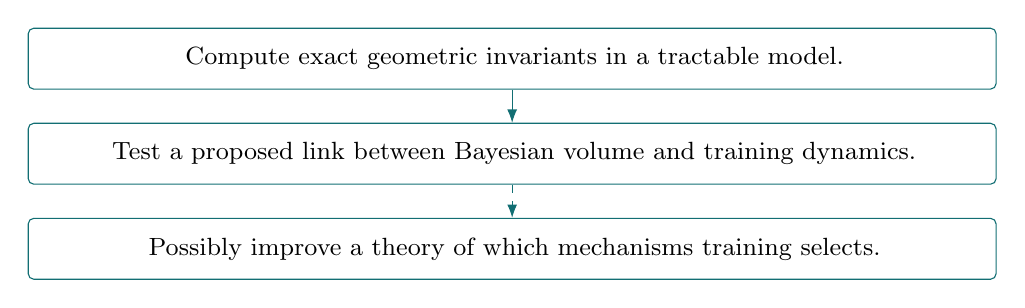
\begin{tikzpicture}[node distance=0.42cm, every node/.style={align=center,font=\small}, box/.style={draw=accent,rounded corners=2pt,inner sep=7pt,text width=11.8cm}, arr/.style={-{Latex},draw=accent}]
\node[box] (a) {Compute exact geometric invariants in a tractable model.};
\node[box,below=of a] (b) {Test a proposed link between Bayesian volume and training dynamics.};
\node[box,below=of b] (c) {Possibly improve a theory of which mechanisms training selects.};
\draw[arr] (a)--(b); \draw[arr,dashed] (b)--(c);
\end{tikzpicture}
\end{center}
\key{Only the first step is the theorem here.} The later arrows require additional mathematics and empirical justification.
\src{[O77], motivation and related problems; [A7], §§1, 3, 6.}
\end{frame}

\begin{frame}[fragile,t,label=slide8]{A limitation worth stating before any theorem}
In the present population model, every exact fit satisfies
\[
BA=\Phi \quad\Longrightarrow\quad BAx=\Phi x\quad\text{for every }x\in\R^I.
\]
Thus different points of the exact-fit fiber do \emph{not} give different predictions on unseen inputs in this model.

Their parameterizations and nearby geometry differ. The model is a test case for proposed theories of selection, not an example of unsafe versus safe predictors on the fiber.

\key{A theorem about this model is not a safety certificate for a deployed AI system.}
\src{Direct consequence of the model; compare the broader motivation in [A7], §1.}
\end{frame}

\begin{frame}[fragile,t,label=slide9]{What MAIS-O77 asks}
For a two-factor linear model with hidden width $H>r=\rk\Phi$:

\textbf{(a)} Compute the local power--logarithmic pair at \emph{every} exact fit $BA=\Phi$. Does it depend only on $(\rk A,\rk B)$? Which strata minimize its first coordinate?

\textbf{(b)} Compute the two-sided pair at \emph{every} point of each specified nonoptimal saddle rung.

The global minimum in (a) is classical reduced-rank regression. The additional targets are the full local table, its equality locus, edge cases, and the saddle statement.
\src{[O77]; [AW05]. The repository page inspected 12 October 2026 still labels the candidate solution as pending review.}
\end{frame}

\begin{frame}[fragile,t,label=slide10]{Context and credit}
\textbf{Classical background:} Aoyagi--Watanabe on reduced-rank regression; Watanabe on singular learning theory.

\textbf{Related geometry:} Lehalleur--Rimányi on multiplication fibers; Lau et al. on the local learning coefficient.

\textbf{Public MAIS contributions:} Sneiderman's overlapping fiber formula and normal form; Novikov's candidate O77 solution and saddle analysis; Brcic's formalization work and specification audits.

\textbf{This blueprint:} a detailed proof and Lean statement-audit package, including an internally proved Wishart identity. No priority claim for previously posted formulas.
\src{[B], §1 and bibliography; [AW05], [LR24], [LFWMW23]; MAIS issues \#3, \#5, \#12.}
\end{frame}

\begin{frame}[fragile,t,label=slide11]{A ``two-layer linear network'' is just two maps}
\begin{center}
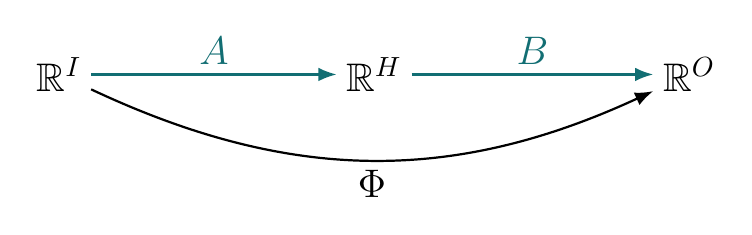
\begin{tikzpicture}[every node/.style={font=\Large},>=Latex]
\node (i) at (0,0) {$\R^I$}; \node (h) at (4,0) {$\R^H$}; \node (o) at (8,0) {$\R^O$};
\draw[->,thick,accent] (i)--node[above]{$A$}(h);
\draw[->,thick,accent] (h)--node[above]{$B$}(o);
\draw[->,thick] (i) to[bend right=25] node[below]{$\Phi$} (o);
\end{tikzpicture}
\end{center}
\[
A\in\Mat HI,\qquad B\in\Mat OH,\qquad
L_\Phi(A,B)=\frac12\Frob{BA-\Phi}^{2}.
\]
The parameter space is $W=\Mat HI\times\Mat OH$, of dimension $H(I+O)$.
The zero set $F_\Phi=L_\Phi^{-1}(0)$ is the multiplication fiber.
\src{[B], Definition 2.1; [O77].}
\end{frame}

\begin{frame}[fragile,t,label=slide12]{Standing notation and geometry}
Throughout the main theorem,
\[
I,O\ge1,\qquad \Phi\in\Mat OI,\qquad r=\rk\Phi<H.
\]
For a fiber point $w=(A,B)$ write $a=\rk A$ and $b=\rk B$.

Every matrix space has its Frobenius norm; $W$ has the Euclidean norm in \emph{all} entries:
\[
\norm{(A,B)}^2=\sum_{i,j}A_{ij}^{2}+\sum_{i,j}B_{ij}^{2}.
\]
Measure always means product Lebesgue measure in those entries, not a measure on the fiber itself.
\src{[B], §§1--2. This convention is subsequently unfolded in Lean.}
\end{frame}

\begin{frame}[fragile,t,label=slide13]{Why this loss occurs in statistics}
Consider the illustrative regression model
\[
x\in\R^I,\quad \mathbb E[xx^{\mathsf T}]=I_I,
\qquad y=\Phi x+\xi,\quad \xi\sim N(0,I_O),
\]
with $\xi$ independent of $x$, and predict $y$ by $BAx$.
The expected excess negative log-likelihood is
\[
\frac12\mathbb E\bigl[\norm{(BA-\Phi)x}^{2}\bigr]
=\frac12\operatorname{tr}\bigl((BA-\Phi)^{\mathsf T}(BA-\Phi)\bigr)
=L_\Phi(A,B).
\]
These statistical assumptions motivate the loss. They are \emph{not extra hypotheses} of the matrix theorem.
\src{[A7], §2.1; Gaussian-regression calculation displayed here.}
\end{frame}

\begin{frame}[fragile,t,label=slide14]{What is training, and what is generalization?}
A training sample is a finite collection $(x_i,y_i)_{i=1}^n$. For our predictor $f_w(x)=BAx$, one empirical loss is
\[
L_n(w)=\frac1{2n}\sum_{i=1}^n\norm{BAx_i-y_i}^2.
\]
Training tries to lower $L_n$, for example by gradient steps
$w_{t+1}=w_t-\eta\nabla L_n(w_t)$. Stochastic gradient descent uses a random subset of the sample to estimate this gradient.

Generalization asks about loss on a new sample from the relevant distribution, not only on the training sample. The population loss is the corresponding expectation.
\src{[A7], §2.1; definitions specialized to the illustrative regression model.}
\end{frame}

\begin{frame}[fragile,t,label=slide15]{Where the Bayesian integral comes from}
A prior density $\varphi(w)$ describes an initial distribution over parameters. In the Gaussian regression example, the likelihood of the observed sample is, up to a parameter-independent factor, $e^{-nL_n(w)}$.

Bayes' rule gives the posterior density
\[
\pi_n(w)=\frac{e^{-nL_n(w)}\varphi(w)}{Z_n},\qquad
Z_n=\int e^{-nL_n(w)}\varphi(w)\,dw.
\]
The normalizing integral is the evidence, up to that same factor.
To isolate the geometry, we next study the analogous integral for the deterministic excess population loss $L_\Phi$.
\src{[W09], [W13]; direct Gaussian-likelihood calculation.}
\end{frame}

\begin{frame}[fragile,t,label=slide16]{Bayesian volume: the deterministic model integral}
Let $U\subset W$ be a fixed bounded neighborhood and $\varphi$ a density bounded above and below there by positive constants. Study
\[
Z_U(n)=\int_U e^{-nL_\Phi(w)}\varphi(w)\,dw,\qquad n\longrightarrow\infty.
\]
It gives greater weight to low loss, but also counts how much parameter volume has that loss.

A smaller volume exponent means a slower decay of $Z_U(n)$, hence greater local mass at the same minimum loss.

\small This is a population-loss Laplace integral. Actual empirical Bayesian evidence is random; its asymptotics require the additional statistical hypotheses of singular learning theory.
\src{[W09], [W13], [LFWMW23]; the bounded-density comparison is elementary.}
\end{frame}

\begin{frame}[fragile,t,label=slide17]{Define the invariant by actual volumes}
For $f:\R^d\to\R$, a point $w$, and $\delta,\eps>0$, put
\[
V_{f,w,\delta}(\eps)=
\vol\{z:\norm{z-w}<\delta,\ |f(z)-f(w)|<\eps\}.
\]
We write $\BP(f,w;\lambda,m)$ when $\lambda\ge0$, $m\in\N$, $m\ge1$, and for \emph{every sufficiently small fixed radius} $\delta$,
\[
V_{f,w,\delta}(\eps)\asymp
\eps^\lambda\bigl(\log(1/\eps)\bigr)^{m-1}
\quad(\eps\downarrow0).
\]
The comparison constants may depend on $w$ and $\delta$, but not on $\eps$.
\src{[B], Definition 2.2; the exact quantifiers will be read in Lecture II.}
\end{frame}

\begin{frame}[fragile,t,label=slide18]{The logarithm is part of the answer}
The notation $F\asymp G$ means two-sided bounds $cG\le F\le CG$ with $0<c\le C<\infty$.
It does \emph{not} assert $F/G\to c_0$.

The pair records
\[
\lambda=\text{power exponent},\qquad m-1=\text{logarithmic degree}.
\]
Thus $(\tfrac12,1)$ and $(\tfrac12,2)$ have the same power but different volumes.

At an exact fit $L_\Phi(w)=0$, the band is the sublevel set $L_\Phi<\eps$. At a saddle, the absolute value must remain.
\src{[B], §2 (definition, conventions, and uniqueness).}
\end{frame}

\begin{frame}[fragile,t,label=slide19]{The regular case: half the number of active variables}
For $f(u)=\norm u^2$ on $\R^d$,
\[
\vol\{u:\norm u^2<\eps\}=\omega_d\eps^{d/2},
\qquad
\int_{\R^d}e^{-n\norm u^2}\,du=\pi^{d/2}n^{-d/2}.
\]
Here $\omega_d$ is the volume of the unit $d$-ball.

If $f(u,z)=\norm u^2$, with $u\in\R^s$ and free variables $z$, then on a small fixed window the pair is
\[
(\lambda,m)=(s/2,1).
\]
The active codimension matters, not the total parameter dimension.
\src{Elementary ball/Gaussian calculations; [B], local-volume calculus (§3).}
\end{frame}

\begin{frame}[fragile,t,label=slide20]{Why the model is singular}
For any $G\in\GL_H(\R)$,
\[
(A,B)\longmapsto(GA,BG^{-1})
\quad\text{preserves }BA.
\]
So parameters are not identifiable: many distinct pairs represent the same linear map.

At rank-deficient pairs, even the rank of the differential
\[
D(BA)_{(A,B)}(\dot A,\dot B)=B\dot A+\dot BA
\]
varies. A single nondegenerate Gaussian approximation cannot describe all points of the zero fiber.
\src{[B], §4; [W09], [W13]. In the derivative, $\dot BA$ means $(\dot B)A$.}
\end{frame}

\begin{frame}[fragile,t,label=slide21]{A crossing produces a logarithm}
Take $f(x,y)=x^2y^2$ at $(0,0)$ in a fixed square $(-a,a)^2$. For $0<\sqrt\eps<a^2$,
\begin{align*}
\vol\{|xy|<\sqrt\eps\}
&=4\int_0^a\min\{a,\sqrt\eps/x\}\,dx\\
&=4\sqrt\eps\left(1+\log\frac{a^2}{\sqrt\eps}\right).
\end{align*}
Hence the pair is $(\tfrac12,2)$ at the crossing, but $(\tfrac12,1)$ at a nonzero point on either axis.

Inscribed and circumscribed squares transfer the same orders to Euclidean balls.
\src{Elementary calculation; compare [A7], §2.2 and [B], the $xy$ calibration in §10.}
\end{frame}

\begin{frame}[fragile,t,label=slide22]{Squaring changes the power, not the logarithmic multiplicity}
For $g(x,y)=xy$,
\[
\vol\{|g|<\eps\}\asymp\eps\log(1/\eps),
\qquad (\lambda,m)=(1,2).
\]
For $f=g^2$,
\[
\vol\{f<\eps\}=\vol\{|g|<\sqrt\eps\}
\asymp\eps^{1/2}\log(1/\eps).
\]
\key{Normalization matters.} The theorem concerns the \emph{squared} Frobenius error. The finite cost will give $2\lambda$, not $\lambda$.
\src{[B], §10 calibration and §2 rank-table definitions.}
\end{frame}

\begin{frame}[fragile,t,label=slide23]{Why the power and logarithm matter statistically}
If a zero-minimum neighborhood has volume pair $(\lambda,m)$, the local Laplace estimate is
\[
Z_U(n)\asymp n^{-\lambda}(\log n)^{m-1}.
\]
Equivalently, its deterministic free energy satisfies
\[
-\log Z_U(n)=\lambda\log n-(m-1)\log\log n+O(1).
\]
At the same minimum loss, smaller $\lambda$ gives more mass asymptotically. At equal $\lambda$, larger $m$ gives more mass.

This explains why the theorem computes both coordinates and then maximizes $m$ on the minimum-$\lambda$ locus. It does not identify Bayesian selection with gradient descent.
\src{[B], §3, Laplace/sublevel comparison; [W09], [W13] for the statistical setting.}
\end{frame}

\begin{frame}[fragile,t,label=slide24]{The geometer's picture: resolution}
\small
In a resolution chart, suppose a nonnegative loss and the pulled-back density have the form
\[
f\circ\pi=u(x)\prod_i|x_i|^{\alpha_i},\qquad
\pi^*(\varphi\,dw)=v(x)\prod_i|x_i|^{\beta_i}\,dx,
\]
where $u,v$ are bounded above and below by positive constants and $\alpha_i>0$ for the relevant divisors.

On such a normal-crossing chart, the candidate power is
\[
\min_i\frac{\beta_i+1}{\alpha_i}.
\]
The logarithmic multiplicity counts simultaneously meeting critical divisors. Across relevant real charts, take the least power and then the largest multiplicity.
\src{[W09], resolution-of-singularities method. This is background, not the formal route used in [B].}
\end{frame}

\begin{frame}[fragile,t,label=slide25]{What is -- and is not -- identified with an RLCT}
For suitable nonnegative real-analytic germs, the volume exponent is the real log canonical threshold (RLCT), related to the leading pole of a local zeta integral.

Here the theorem is formulated directly as
\[
\BP(L_\Phi,w;\lambda,m).
\]
\key{The formal conclusion is two-sided radius-first bounds.} It does not include a formal meromorphic continuation theorem or an exact leading asymptotic constant.

At saddles, call this a \emph{signed-band pair}; do not silently import the Bayesian interpretation of a local minimum.
\src{[B], abstract, §2 and §7; [W09], [LFWMW23].}
\end{frame}

\begin{frame}[fragile,t,label=slide26]{Bayesian selection is not gradient descent}
Volume-weighted integrals and trajectories answer different questions:
\[
\int e^{-nL(w)}\varphi(w)\,dw
\qquad\hbox{versus}\qquad
\dot w=-\nabla L(w).
\]
Stochastic gradient descent adds noise, but it is not automatically a reversible Langevin process with a Gibbs stationary law.

The proposed ``opposing staircases'' link is something to test, not a premise we are allowed to assume.

At a saddle, the set $\{L<L(w)+\eps\}$ already contains lower-loss regions; the two-sided shrinking band is a genuinely different object.
\src{[A7], §§2.1, 3 and 6; [O77].}
\end{frame}

\begin{frame}[fragile,t,label=slide27]{The result we will eventually read in Lean}
\small
At an exact fit of ranks $(a,b)$ set
\[
p=O-b,\quad q=I-a,\quad h=H+r-a-b,\quad s=Oa+b(I-a).
\]
For the integers $0\le t\le\min(h,q)$, put $c(t)=(h-t)(q-t)+pt$. Then
\[
\boxed{\qquad \lambda=\frac{s+\min_t c(t)}2,
\qquad m=\#\arg\min_t c(t).\qquad}
\]
The minimization is over integers. The theorem also classifies all minimizing rank strata and proves pair $(1,1)$ on every specified nonoptimal saddle rung.
\src{[B], main theorem (label thm:main-answer) and §§7--10.}
\end{frame}

\begin{frame}[fragile,t,label=slide28]{The question before the proof}
\vspace{0.6cm}
{\Large Is the formal statement really saying this?}\par
\vspace{0.5cm}
We must check the measure, the loss, the order of limits, natural-number subtraction, rank constraints, and all universal quantifiers.

Only after that does a proof checker answer the question we intended to ask.
\src{[B], §2.3; [Lean-Check], distinction between proof validity and statement meaning.}
\end{frame}

\section[Lecture II]{A first Lean audit: entries, measures, and bands}
\renewcommand{\lecturetag}{Lecture II}

\begin{frame}[fragile,t,label=lectureII]{A first Lean audit: entries, measures, and bands}
\vspace{0.9cm}{\Large\color{accent}Lecture II}\par\vspace{0.5cm}{\LARGE Read definitions before trusting the theorem name.}
\end{frame}

\begin{frame}[fragile,t,label=slide30]{The final theorem: a first look}
\leancontext{O77}
\begin{lstlisting}[style=lean]
theorem answersO77 {I O H : ℕ} (Phi : Matrix (Fin O) (Fin I) ℝ)
    (hI : 0 < I) (hO : 0 < O) (hrH : Phi.rank < H) : AnswersO77 (H := H) Phi :=
  answersO77_of_wishart GlobalSpectralIntegral.realWishartEigenvalueFormula
    Phi hI hO hrH
\end{lstlisting}

\translation{For every $I,O,H\in\N$ and every real $O\times I$ matrix $\Phi$, if $I>0$, $O>0$, and $\rk\Phi<H$, then the proposition \node{AnswersO77 (H := H) Phi} holds.}
\auditnote{At this stage, the name \node{AnswersO77} is opaque to us. Knowing its name is not knowing what has been proved.}
\src{[B], §2.3; source lines 1012--1015. We will unpack its full proposition in Lecture IV.}
\end{frame}

\begin{frame}[fragile,t,label=slide31]{A proposition is a type; a proof is a term}
\key{A teaching example, not a blueprint quotation:}
\begin{lstlisting}[style=lean]
example (P Q : Prop) (h : P ∧ Q) : Q ∧ P :=
  ⟨h.2, h.1⟩
\end{lstlisting}

\translation{For any propositions $P,Q$, a proof of $P\land Q$ supplies a proof of $Q\land P$. The pair of proofs is reordered.}
\small
\node{Prop} is the type of propositions. In \node{h : P}, the object $h$ is a proof of $P$; the colon does not mean a numerical assignment.
\src{[Lean-T], propositions and proofs; [B], §2.3 notation guide.}
\end{frame}

\begin{frame}[fragile,t,label=slide32]{Proof terms and tactic scripts have the same endpoint}
\key{The same teaching example, with tactics:}
\begin{lstlisting}[style=lean]
example (P Q : Prop) (h : P ∧ Q) : Q ∧ P := by
  constructor
  · exact h.2
  · exact h.1
\end{lstlisting}

\translation{To prove a conjunction, prove its two factors. First use the proof of $Q$, then the proof of $P$.}
The tactics construct a proof term. In the usual checking path, the kernel checks that term rather than trusting an English account of the tactic's intention.
\src{[Lean-T], tactics; [Lean-Elab], elaboration and kernel checking.}
\end{frame}

\begin{frame}[fragile,t,label=slide33]{Read a declaration at the colon}
\begin{tabular}{@{}p{.43\textwidth}p{.51\textwidth}@{}}
\node{def name (...) : T := value} & Defines an object of type $T$.\\[10pt]
\node{def name (...) : Prop := P} & Defines a \emph{predicate}; it does not prove $P$.\\[10pt]
\node{theorem name (...) : P := proof} & Provides a proof of $P$, under the listed arguments.\\[10pt]
\node{structure S ... where ...} & Defines a record type with named fields. Fields can be data or proof obligations.
\end{tabular}
\vspace{0.3cm}
For a statement audit, first read everything before \node{:=}; then unfold every nonstandard predicate it names.
\src{[B], §2.3; [Lean-T], dependent types and structures.}
\end{frame}

\begin{frame}[fragile,t,label=slide34]{Three kinds of brackets}
\begin{tabular}{@{}p{.36\textwidth}p{.58\textwidth}@{}}
\node{(Phi : RM O I)} & An explicit argument: supply the target matrix.\\[11pt]
\node{{I O H : ℕ}} & Implicit arguments: still universally quantified, but usually inferred.\\[11pt]
\node{[Fintype ι]} & A type-class instance: here it provides a finite enumeration of the index type $\iota$.
\end{tabular}
\vspace{0.3cm}
\node{(H := H)} supplies one implicit argument by name. It prevents an ambiguity; it does not add an assumption.

\small Braces around a set, such as \node{{x | P x}}, have a different role: set comprehension.
\src{[B], §2.3 notation guide.}
\end{frame}

\begin{frame}[fragile,t,label=slide35]{Namespaces and notation are part of the audit}
The short name \node{loss} below resolves to \node{O77.Native.loss}.
The short name \node{RadiusOrder} resolves to \node{O77.Transport0906.RadiusOrder}.

The source opens namespaces to avoid repeating long names. A declaration may also sit inside a \node{noncomputable section}.

\key{Do not infer meaning from the spelling of a short name alone.} Follow its actual resolution and the type-class instances supplying operations.

\small These slides name the relevant namespace and cite the source. They do not reproduce every import, scope command, or library instance.
\src{[B], §2.3 and preservation/audit notes; [Lean-Check].}
\end{frame}

\begin{frame}[fragile,t,label=slide36]{Finite indices, matrices, and products}
\[
\node{Fin n}\quad\longleftrightarrow\quad\{0,1,\ldots,n-1\}.
\]
A matrix type \node{Matrix m n ℝ} is a function type $m\to n\to\R$. Here $m,n$ are index types, not necessarily natural numbers.

For dimension indices we use \node{Matrix (Fin O) (Fin I) ℝ}.
Multiplication is finite matrix multiplication, and \node{A.rank} is the real linear rank.

For $w=(A,B)$, \node{w.1} is $A$, \node{w.2} is $B$. Therefore \node{w.2 * w.1} is $BA$, in that order.
\src{[B], §2.3 notation guide; Mathlib matrix conventions cited in [B].}
\end{frame}

\begin{frame}[fragile,t,label=declRM]{The parameter type}
\leancontext{O77.Reconstruction0905 (RM); O77.Native (Parameters)}
\begin{lstlisting}[style=lean]
abbrev RM (m n : Nat) := Matrix (Fin m) (Fin n) ℝ

abbrev Parameters (I O H : ℕ) := RM H I × RM O H
\end{lstlisting}
\translation{
For $m,n\in\N$, $\mathrm{RM}(m,n)=\R^{m\times n}$.
For $I,O,H\in\N$,
\[
\mathrm{Parameters}(I,O,H)=\R^{H\times I}\times\R^{O\times H}.
\]
A point is ordered as $(A,B)$, even though the represented map is $BA$.
}
\src{[B], §2.3; declaration start line(s) 657, 659.}
\end{frame}

\begin{frame}[fragile,t,label=declfrobeniusSq]{The squared Frobenius norm}
\leancontext{O77.Residual}
\begin{lstlisting}[style=lean]
def frobeniusSq {m n : Type*} [Fintype m] [Fintype n]
    (A : Matrix m n ℝ) : ℝ :=
  ∑ i, ∑ j, (A i j) ^ 2
\end{lstlisting}
\translation{
For any finite index types $m,n$ and $A:m\times n\to\R$,
\[
\mathrm{frobeniusSq}(A)=\sum_{i\in m}\sum_{j\in n} A_{ij}^2=\Frob A^2.
\]
The symbols $m,n$ here name finite \emph{types}. The brackets supply their finite enumerations.
}
\src{[B], §2.3; declaration start line(s) 672.}
\end{frame}

\begin{frame}[fragile,t,label=declcoordinateLebesgue]{Lebesgue measure in a finite coordinate space}
\leancontext{O77.Residual}
\begin{lstlisting}[style=lean]
noncomputable def coordinateLebesgue ( ι : Type*) [Fintype ι] :
    MeasureTheory.Measure ( ι → ℝ) :=
  MeasureTheory.Measure.pi fun _ : ι => MeasureTheory.volume
\end{lstlisting}
\translation{
For any finite index type $\iota$, equip $\R^\iota$ with
\[
\mathrm{coordinateLebesgue}(\iota)=\bigotimes_{i\in\iota}dx_i.
\]
\node{Measure.pi} means finite product measure; \node{volume} on $\R$ is Lebesgue measure.
}
\auditnote{\node{noncomputable} does not mean unproved. It says an executable computation is not being supplied.}
\src{[B], §2.3; declaration start line(s) 676.}
\end{frame}

\begin{frame}[fragile,t,label=declmatrixLebesgue]{Lebesgue measure in every matrix entry}
\leancontext{O77.Residual}
\begin{lstlisting}[style=lean]
noncomputable def matrixLebesgue (p h : Type*) [Fintype p] [Fintype h] :
    MeasureTheory.Measure (Matrix p h ℝ) :=
  MeasureTheory.Measure.pi fun _ : p => coordinateLebesgue h
\end{lstlisting}
\translation{
For finite index types $p,h$, the matrix space has measure
\[
\bigotimes_{i\in p}\left(\bigotimes_{j\in h}dA_{ij}\right).
\]
The outer product is over rows, the inner product over columns. Empty products give the one-point measure of mass $1$.
}
\auditnote{This is an ambient entry measure, not a Hausdorff measure on a rank stratum.}
\src{[B], §2.3; declaration start line(s) 680.}
\end{frame}

\begin{frame}[fragile,t,label=declentryMeasure]{The measure on pairs of matrices}
\leancontext{O77.Native}
\begin{lstlisting}[style=lean]
def entryMeasure (I O H : ℕ) : Measure (Parameters I O H) :=
  (matrixLebesgue (Fin H) (Fin I)).prod (matrixLebesgue (Fin O) (Fin H))
\end{lstlisting}
\translation{
For dimensions $I,O,H\in\N$,
\[
d\mu_W(A,B)=
\left(\prod_{i=1}^{H}\prod_{j=1}^{I}dA_{ij}\right)
\left(\prod_{i=1}^{O}\prod_{j=1}^{H}dB_{ij}\right).
\]
\node{.prod} is binary product measure. No free measure argument remains in the theorem.
}
\src{[B], §2.3; declaration start line(s) 695.}
\end{frame}

\begin{frame}[fragile,t,label=declambientSq]{The actual Euclidean norm}
\leancontext{O77.Native}
\begin{lstlisting}[style=lean]
def ambientSq {I O H : ℕ} (w : Parameters I O H) : ℝ :=
  frobeniusSq w.1 + frobeniusSq w.2

def entryNorm {I O H : ℕ} (w : Parameters I O H) : ℝ :=
  Real.sqrt (ambientSq w)
\end{lstlisting}
\translation{
For $w=(A,B)$,
\[
\mathrm{ambientSq}(w)=\Frob A^2+\Frob B^2,
\qquad \mathrm{entryNorm}(w)=\sqrt{\Frob A^2+\Frob B^2}.
\]
This explicitly chooses the Euclidean norm in all entries.
}
\auditnote{An unrelated default norm on function types cannot silently redefine the balls.}
\src{[B], §2.3; declaration start line(s) 698, 701.}
\end{frame}

\begin{frame}[fragile,t,label=declloss]{The loss, with its normalization visible}
\leancontext{O77.Native}
\begin{lstlisting}[style=lean]
def loss {I O H : ℕ} (Phi : RM O I) (w : Parameters I O H) : ℝ :=
  frobeniusSq (w.2 * w.1 - Phi) / 2
\end{lstlisting}
\translation{
For every target $\Phi\in\R^{O\times I}$ and parameter $w=(A,B)$,
\[
\mathrm{loss}(\Phi,w)=L_\Phi(A,B)=\frac12\sum_{i,j}\bigl((BA)_{ij}-\Phi_{ij}\bigr)^2.
\]
This is a total, nonnegative polynomial function of the entries, with zero set $F_\Phi$.
}
\src{[B], §2.3; declaration start line(s) 704.}
\end{frame}

\begin{frame}[fragile,t,label=declentryBall]{The fixed spatial window}
\leancontext{O77.Native}
\begin{lstlisting}[style=lean]
def entryBall {I O H : ℕ} (w : Parameters I O H) (R : ℝ) : Set (Parameters I O H) :=
  {v | entryNorm (v-w) < R}
\end{lstlisting}
\translation{
For $w\in W$ and $R\in\R$,
\[
\mathrm{entryBall}(w,R)=\{v\in W:\norm{v-w}<R\}.
\]
It is an open Euclidean ball when $R>0$. The definition makes sense for every real $R$; later hypotheses require positive radii.
}
\src{[B], §2.3; declaration start line(s) 707.}
\end{frame}

\begin{frame}[fragile,t,label=declbandSet]{The band is centered at the actual loss value}
\leancontext{O77.Native}
\begin{lstlisting}[style=lean]
def bandSet {I O H : ℕ} (Phi : RM O I) (w : Parameters I O H) (R eps : ℝ) :
    Set (Parameters I O H) :=
  {v | v ∈ entryBall w R ∧ |loss Phi v - loss Phi w| < eps}
\end{lstlisting}
\translation{
For $\Phi,w,R,\eps$ of the displayed types,
\[
\mathrm{bandSet}(\Phi,w,R,\eps)=
\{v\in W:\norm{v-w}<R,\ |L_\Phi(v)-L_\Phi(w)|<\eps\}.
\]
At an exact fit this is $L_\Phi(v)<\eps$ inside the ball; otherwise the centering and absolute value remain.
}
\auditnote{No equation $L_\Phi(w)=0$ is built into this definition.}
\src{[B], §2.3; declaration start line(s) 710.}
\end{frame}

\begin{frame}[fragile,t,label=declbandVolume]{The observable being estimated}
\leancontext{O77.Native}
\begin{lstlisting}[style=lean]
def bandVolume {I O H : ℕ} (Phi : RM O I) (w : Parameters I O H) (R eps : ℝ) : ENNReal :=
  entryMeasure I O H (bandSet Phi w R eps)
\end{lstlisting}
\translation{
\[
\mathrm{bandVolume}(\Phi,w,R,\eps)
=\mu_W\bigl(\mathrm{bandSet}(\Phi,w,R,\eps)\bigr).
\]
The codomain \node{ENNReal} is $[0,+\infty]$. For positive finite $R$, this particular measure is finite because the band is contained in a bounded ball.
}
\src{[B], §2.3; declaration start line(s) 714.}
\end{frame}

\begin{frame}[fragile,t,label=slide47]{Why use extended nonnegative reals?}
A measure takes values in $[0,+\infty]$, even before finiteness has been proved.

For a real number $x$,
\[
\node{ENNReal.ofReal x}=\max\{x,0\}\quad\text{viewed in }[0,+\infty].
\]
In the asymptotic comparison, $c,C,\eps$ and $\log(1/\eps)$ are positive. Thus the conversions introduce no truncation of the quantities being compared.

\key{Audit principle:} check positivity before identifying extended-real expressions with ordinary real inequalities.
\src{[B], §2.3, measure and power--logarithm paragraphs.}
\end{frame}

\begin{frame}[fragile,t,label=declpowerLogZeroReal]{The comparison function}
\leancontext{O77.Residual}
\begin{lstlisting}[style=lean]
def powerLogZeroReal (lam : Real) (k : Nat) (eps : Real) : Real :=
  eps ^ lam * (Real.log (1 / eps)) ^ k

def powerLogZero (lam : Real) (k : Nat) (eps : Real) : ENNReal :=
  ENNReal.ofReal (powerLogZeroReal lam k eps)
\end{lstlisting}
\translation{
For $\lambda\in\R$, $k\in\N$, and $\eps>0$, put
\[
g_{\lambda,k}(\eps)=\eps^\lambda\bigl(\log(1/\eps)\bigr)^k.
\]
The first definition is real-valued; the second embeds its nonnegative part into $[0,+\infty]$. We will only test it for $0<\eps<e^{-1}$.
}
\auditnote{\node{eps ^ lam} uses real power; the logarithm raised to \node{k : Nat} uses ordinary integer power.}
\src{[B], §2.3; declaration start line(s) 739, 742.}
\end{frame}

\begin{frame}[fragile,t,label=declEThetaZeroPowerLog]{Two-sided bounds at one fixed radius}
\leancontext{O77.Residual}
\begin{lstlisting}[style=lean,basicstyle=\ttfamily\fontsize{8.1}{10.1}\selectfont]
def EThetaZeroPowerLog (V : Real -> ENNReal) (lam : Real) (k : Nat) : Prop :=
  ∃ c C eps0 : Real,
    0 < c ∧ c ≤ C ∧ 0 < eps0 ∧ eps0 < Real.exp (-1) ∧
      ∀ eps : Real, 0 < eps -> eps < eps0 ->
        ENNReal.ofReal c * powerLogZero lam k eps ≤ V eps ∧
          V eps ≤ ENNReal.ofReal C * powerLogZero lam k eps
\end{lstlisting}
\translation{
For $V:\R\to[0,+\infty]$, the predicate says that there exist real $c,C,\eps_0$ with
\[
0<c\le C,\quad 0<\eps_0<e^{-1},\quad
c\eps^\lambda\log(1/\eps)^k\le V(\eps)\le C\eps^\lambda\log(1/\eps)^k
\]
for every $0<\eps<\eps_0$.
}
\auditnote{The constants are chosen before the universally quantified $\eps$.}
\src{[B], §2.3; declaration start line(s) 745.}
\end{frame}

\begin{frame}[fragile,t,label=slide50]{Read the quantifiers in their actual order}
For one fixed radius, the declaration says
\[
\exists(c,C,\eps_0)\quad\forall\eps\in(0,\eps_0)\quad\text{the bounds hold}.
\]
It does \emph{not} say
\[
\forall\eps\quad\exists(c_\eps,C_\eps)\quad\text{the bounds hold}.
\]
The second statement would usually say almost nothing about asymptotic order.

\key{A proof assistant checks the quantifiers written, not the quantifiers intended.}
\src{[B], §2.3; direct logical comparison of the two specifications.}
\end{frame}

\begin{frame}[fragile,t,label=declRadiusOrder]{The radius-first wrapper}
\leancontext{O77.Transport0906}
\begin{lstlisting}[style=lean]
def RadiusOrder (V : ℝ → ℝ → ENNReal) (lam : ℝ) (m : ℕ) : Prop :=
  0 ≤ lam ∧ 1 ≤ m ∧ ∃ rho : ℝ, 0 < rho ∧
    ∀ delta, 0 < delta → delta < rho →
      EThetaZeroPowerLog (V delta) lam (m-1)
\end{lstlisting}
\translation{
For $V:\R\to\R\to[0,+\infty]$, $\lambda\in\R$, and $m\in\N$,
\[
\lambda\ge0,\quad m\ge1,\quad
\exists\rho>0\ \forall\delta\in(0,\rho):\
V(\delta,\eps)\asymp\eps^\lambda\log(1/\eps)^{m-1}.
\]
The comparison constants and the cutoff for $\eps$ may depend on $\delta$.
}
\auditnote{The radius is fixed first. This is not an asymptotic along $\delta=\delta(\eps)$.}
\src{[B], §2.3; declaration start line(s) 763.}
\end{frame}

\begin{frame}[fragile,t,label=slide52]{Expand the complete order of limits once}
The core quantified assertion is
\begin{gather*}
\exists\rho>0\quad\forall\delta\in(0,\rho)\quad
\exists c_\delta,C_\delta,\eps_\delta,\\[4pt]
0<c_\delta\le C_\delta<\infty,\qquad 0<\eps_\delta<e^{-1},\\[4pt]
\forall\eps\in(0,\eps_\delta),\\[2pt]
c_\delta\eps^\lambda\log(1/\eps)^{m-1}
\le V_{L_\Phi,w,\delta}(\eps)
\le C_\delta\eps^\lambda\log(1/\eps)^{m-1}.
\end{gather*}
Both powers describe the same germ, independently of the sufficiently small fixed ball chosen.
\src{[B], Definition 2.2 and §2.3.}
\end{frame}

\begin{frame}[fragile,t,label=slide53]{Natural-number subtraction has a trap}
In Lean, subtraction in $\N$ is truncated:
\[
(2-5:\N)=0,\qquad (2:\Z)-5=-3.
\]
Thus \node{m - 1} would be $0$ both at $m=0$ and at $m=1$.
The guard \node{1 ≤ m} in \node{RadiusOrder} removes this ambiguity.

We must also guard $O-b$, $I-a$, and $H+r-(a+b)$ before interpreting them as dimensions. The rank structure will do exactly that.
\src{[B], §2.3, arithmetic and radius-wrapper explanations.}
\end{frame}

\begin{frame}[fragile,t,label=declHasLocalBandPair]{The geometric predicate, finally assembled}
\leancontext{O77.Native}
\begin{lstlisting}[style=lean]
def HasLocalBandPair {I O H : ℕ} (Phi : RM O I) (w : Parameters I O H)
    (lam : ℝ) (m : ℕ) : Prop :=
  RadiusOrder (bandVolume Phi w) lam m
\end{lstlisting}
\translation{
\[
\mathrm{HasLocalBandPair}(\Phi,w,\lambda,m)
\quad\Longleftrightarrow\quad
\BP(L_\Phi,w;\lambda,m)
\]
with the explicit entry measure, Euclidean balls, two-sided bands, and radius-first quantifiers just read.
}
\auditnote{There is no rank formula, normal-form hypothesis, or assumed asymptotic result inside this definition.}
\src{[B], §2.3; declaration start line(s) 780.}
\end{frame}

\begin{frame}[fragile,t,label=slide55]{The statement dependency chain so far}
\begin{center}
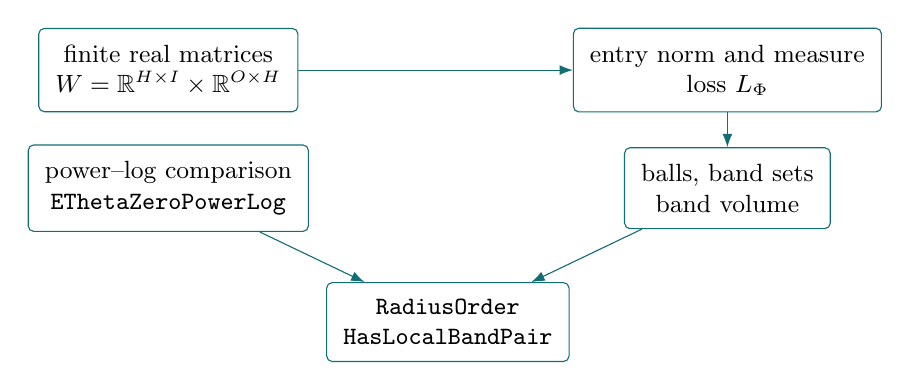
\begin{tikzpicture}[every node/.style={align=center,font=\small}, box/.style={draw=accent,rounded corners=2pt,inner sep=6pt},>=Latex]
\node[box] (a) at (0,2.4) {finite real matrices\\$W=\Mat HI\times\Mat OH$};
\node[box] (b) at (7.1,2.4) {entry norm and measure\\loss $L_\Phi$};
\node[box] (c) at (7.1,0.9) {balls, band sets\\band volume};
\node[box] (d) at (0,0.9) {power--log comparison\\\node{EThetaZeroPowerLog}};
\node[box] (e) at (3.55,-.8) {\node{RadiusOrder}\\\node{HasLocalBandPair}};
\draw[->,accent] (a)--(b);\draw[->,accent] (b)--(c);
\draw[->,accent] (c)--(e);\draw[->,accent] (d)--(e);
\end{tikzpicture}
\end{center}
No analytical proof has been read; the observable itself is now specified.
\src{[B], §2.3. Arrows indicate statement dependencies, not proof dependencies.}
\end{frame}

\begin{frame}[fragile,t,label=slide56]{The pair is unique -- if it exists}
Suppose two pairs describe the same germ. On a common fixed ball, divide their bounds to obtain
\[
c\le\eps^{\lambda-\lambda'}\log(1/\eps)^{m-m'}\le C.
\]
Set $t=\log(1/\eps)$ and take logarithms:
\[
-(\lambda-\lambda')t+(m-m')\log t=O(1).
\]
First divide by $t$; then compare the remaining logarithm. Hence $\lambda=\lambda'$ and $m=m'$.

\small For a locally constant germ, the convention is $(0,1)$; it does not assign a zeta pole to the zero function.
\src{[B], uniqueness and constant-germ lemma (§2).}
\end{frame}

\begin{frame}[fragile,t,label=slide57]{What we have checked -- and what is still missing}
We now know what the formal sentence
\[
\node{HasLocalBandPair Phi w lam m}
\]
means, without relying on its suggestive name.

What remains is to read the \emph{numerical candidate}, the \emph{geometric domain}, and the six claims that connect those candidates to actual volumes.

\key{Defining an invariant is not computing it.}
\src{[B], §2.3 statement-audit structure.}
\end{frame}

\section[Lecture III]{The full table on the exact-fit fiber}
\renewcommand{\lecturetag}{Lecture III}

\begin{frame}[fragile,t,label=lectureIII]{The full table on the exact-fit fiber}
\vspace{0.9cm}{\Large\color{accent}Lecture III}\par\vspace{0.5cm}{\LARGE From seven rank inequalities to every local pair}
\end{frame}

\begin{frame}[fragile,t,label=slide59]{Which rank pairs can occur?}
Fix $\Phi$ of rank $r$, and let $a=\rk A$, $b=\rk B$ at an exact fit.
The feasible pairs are exactly
\[
r\le a\le\min(H,I),\qquad r\le b\le\min(H,O),\qquad a+b\le H+r.
\]
The first inequalities come from $BA=\Phi$. The last is Sylvester's rank inequality.

The converse is part of the result: every such pair is realized over this \emph{fixed} target $\Phi$, not merely over some matrix of rank $r$.
\src{[B], §4, rank-feasibility lemma; main theorem, clause 2.}
\end{frame}

\begin{frame}[fragile,t,label=declRankData]{A proposition-valued structure}
\leancontext{O77}
\begin{lstlisting}[style=lean,basicstyle=\ttfamily\fontsize{8.2}{10.2}\selectfont]
structure RankData (I O H r a b : Nat) : Prop where
  r_le_a : r ≤ a
  r_le_b : r ≤ b
  a_le_I : a ≤ I
  a_le_H : a ≤ H
  b_le_O : b ≤ O
  b_le_H : b ≤ H
  sum_le : a + b ≤ H + r
\end{lstlisting}
\translation{
\node{RankData I O H r a b} is the conjunction of the seven displayed inequalities.
Its fields are \emph{proofs}, not additional numerical data.

Thus a term of this type certifies that $(a,b)$ is feasible for dimensions $(I,O,H)$ and target rank $r$.
}
\src{[B], §2.3; declaration start line(s) 797.}
\end{frame}

\begin{frame}[fragile,t,label=slide61]{Why the last inequality is necessary}
The restriction $B|_{\im A}$ has rank $r$, so
\[
\dim(\im A\cap\ker B)=a-r.
\]
Since $\dim\ker B=H-b$, we obtain $a-r\le H-b$.

Conversely, choose subspaces with the prescribed dimensions: $r$ transmitted directions, $a-r$ directions killed by $B$, and $b-r$ directions not reached by $A$. A change of input and output bases then realizes the given $\Phi$.

\key{All rank conditions are elementary linear algebra.}
\src{[B], §4, feasibility and simultaneous normal-form lemmas.}
\end{frame}

\begin{frame}[fragile,t,label=declresidualHidden]{Two dimensions appearing in the local model}
\leancontext{O77}
\begin{lstlisting}[style=lean]
def residualHidden (H r a b : Nat) : Nat := (H + r) - (a + b)

def regularDim (I O a b : Nat) : Nat := O * a + b * (I - a)
\end{lstlisting}
\translation{
For a feasible pair, define
\[
h=H+r-a-b,\qquad s=Oa+b(I-a).
\]
The residual matrix product has hidden dimension $h$. The regular quadratic part has $s$ coordinates.

Also put $p=O-b$ and $q=I-a$.
}
\auditnote{Feasibility ensures $a\le I$, $b\le O$, and $a+b\le H+r$, so these natural-number subtractions are ordinary dimension differences.}
\src{[B], §2.3; declaration start line(s) 806, 807.}
\end{frame}

\begin{frame}[fragile,t,label=slide63]{The normal form predicts the shape of the answer}
Near an exact fit of ranks $(a,b)$, suitable real-analytic coordinates give
\[
L_\Phi\asymp\norm{u}^2+\Frob{YZ}^{2},\qquad
u\in\R^s,\quad Y\in\R^{p\times h},\quad Z\in\R^{h\times q},
\]
with additional free coordinates and a Jacobian bounded above and below.

Here
\[
p=O-b,\quad q=I-a,\quad h=H+r-a-b,\quad s=OI-pq.
\]
Each regular quadratic coordinate contributes $1/2$ to $\lambda$; the remaining calculation is at the zero matrix product.
\src{[B], §5 (elimination chart) and §9. The loss comparison is not an assertion of equality in an isometric chart.}
\end{frame}

\begin{frame}[fragile,t,label=slide64]{A finite quadratic controls the residual product}
For $p,q,h\in\N$, consider
\[
c_{p,q,h}(t)=(h-t)(q-t)+pt
=hq+t^2-(h+q-p)t,
\quad 0\le t\le\min(h,q),\ t\in\Z.
\]
Define
\[
d_0(p,q,h)=\min_t c_{p,q,h}(t),\qquad
\mu_0(p,q,h)=\#\{t:c_{p,q,h}(t)=d_0(p,q,h)\}.
\]
The residual pair will be $(d_0/2,\mu_0)$.

\key{Next we read the actual finite minimum in Lean.}
\src{[B], Definition 2.3 and §7.}
\end{frame}

\begin{frame}[fragile,t,label=slide65]{The finite cost already has a geometric meaning}
For the zero-product fiber, stratify by the rank $t$ of $Z$:
\[
\Sigma_t=\{(Y,Z):YZ=0,\ \rk Z=t\}.
\]
The rank-$t$ stratum of $h\times q$ matrices has codimension $(h-t)(q-t)$. For each such $Z$, requiring $Y$ to vanish on $\im Z$ imposes $pt$ independent linear conditions.
Hence
\[
\codim\Sigma_t=(h-t)(q-t)+pt=c_{p,q,h}(t).
\]
So $d_0$ is the codimension of the zero-product fiber. The analytic theorem proves that its learning exponent is $d_0/2$; that relation is not automatic for an arbitrary nonnegative polynomial.
\src{Rank-stratum dimension and linear constraint count; compare [B], §§4, 7 and [LR24].}
\end{frame}

\begin{frame}[fragile,t,label=declresidualCost]{The nonnegative cost expression}
\leancontext{O77}
\begin{lstlisting}[style=lean]
def residualCost (p q h t : Nat) : Nat := (h - t) * (q - t) + p * t
\end{lstlisting}
\translation{
On the range $0\le t\le\min(h,q)$,
\[
\mathrm{residualCost}(p,q,h,t)=(h-t)(q-t)+pt=c_{p,q,h}(t).
\]
Outside that range the two subtractions are truncated in $\N$.
The polynomial identity with $hq+t^2-(h+q-p)t$ is used only on the allowed range.
}
\src{[B], §2.3; declaration start line(s) 844.}
\end{frame}

\begin{frame}[fragile,t,label=declquadratic]{An integer polynomial, not truncated subtraction}
\leancontext{O77.Arithmetic}
\begin{lstlisting}[style=lean]
def quadratic (B D : Int) (t : Nat) : Int :=
  B + (t : Int) * (t : Int) - D * (t : Int)
\end{lstlisting}
\translation{
For integers $B,D$ and a natural-number index $t$,
\[
\mathrm{quadratic}(B,D,t)=B+t^2-Dt\in\Z.
\]
Here $B$ is a scalar coefficient, unrelated to the factor matrix $B$.
The explicit casts \node{(t : Int)} place all arithmetic in $\Z$.
}
\src{[B], §2.3; declaration start line(s) 826.}
\end{frame}

\begin{frame}[fragile,t,label=declresidualQuadratic]{The polynomial used by the finite search}
\leancontext{O77}
\begin{lstlisting}[style=lean]
def residualQuadratic (p q h : Nat) : Nat → Int :=
  Arithmetic.quadratic ((h : Int) * (q : Int))
    ((h : Int) + (q : Int) - (p : Int))
\end{lstlisting}
\translation{
For $p,q,h\in\N$,
\[
\mathrm{residualQuadratic}(p,q,h)(t)=hq+t^2-(h+q-p)t\in\Z.
\]
The coefficient $h+q-p$ may be negative. Its definition is integer arithmetic, which preserves that sign.
}
\auditnote{On $0\le t\le\min(h,q)$, this equals the preceding natural-valued cost after casting to $\Z$.}
\src{[B], §2.3; declaration start line(s) 846.}
\end{frame}

\begin{frame}[fragile,t,label=declminimumUpTo]{A recursive minimum over an inclusive interval}
\leancontext{O77.Arithmetic}
\begin{lstlisting}[style=lean]
def minimumUpTo (f : Nat → Int) : Nat → Int
  | 0 => f 0
  | K + 1 => min (minimumUpTo f K) (f (K + 1))
\end{lstlisting}
\translation{
For $f:\N\to\Z$, recursion defines
\[
M_f(0)=f(0),\qquad M_f(K+1)=\min\{M_f(K),f(K+1)\}.
\]
Induction gives $M_f(K)=\min\{f(0),\ldots,f(K)\}$.

The endpoint $K$ is included, and the set is never empty.
}
\src{[B], §2.3; declaration start line(s) 829.}
\end{frame}

\begin{frame}[fragile,t,label=declminimizerList]{All minimizers, with no duplicates}
\leancontext{O77.Arithmetic}
\begin{lstlisting}[style=lean]
def minimizerList (f : Nat → Int) (K : Nat) : List Nat :=
  (List.range (K + 1)).filter (fun t => decide (f t = minimumUpTo f K))
\end{lstlisting}
\translation{
\node{List.range (K + 1)} is the list $[0,1,\ldots,K]$.
Filtering it retains precisely those $t$ for which $f(t)=M_f(K)$.

\node{decide} converts a decidable proposition to a Boolean test used by the filter. Equality of integers is decidable.

The result is a list of every minimizing index, each appearing once.
}
\src{[B], §2.3; declaration start line(s) 833.}
\end{frame}

\begin{frame}[fragile,t,label=declresidualMin]{The residual minimum itself}
\leancontext{O77}
\begin{lstlisting}[style=lean]
def residualMin (p q h : Nat) : Nat :=
  (Arithmetic.minimumUpTo (residualQuadratic p q h) (min h q)).toNat
\end{lstlisting}
\translation{
Compute the integer minimum of $hq+t^2-(h+q-p)t$ for $t=0,\ldots,\min(h,q)$, then convert it to $\N$.

Every cost on this range is nonnegative, because it also equals $(h-t)(q-t)+pt$. Thus the integer minimum is nonnegative, and \node{.toNat} preserves it:
\[
\mathrm{residualMin}(p,q,h)=d_0(p,q,h).
\]
}
\auditnote{Without the nonnegativity argument, \node{Int.toNat} could silently replace a negative result by zero.}
\src{[B], §2.3; declaration start line(s) 850.}
\end{frame}

\begin{frame}[fragile,t,label=declresidualMinimizerList]{Multiplicity is a count of minimizing indices}
\leancontext{O77}
\begin{lstlisting}[style=lean]
def residualMinimizerList (p q h : Nat) : List Nat :=
  Arithmetic.minimizerList (residualQuadratic p q h) (min h q)

def residualMultiplicity (p q h : Nat) : Nat :=
  (residualMinimizerList p q h).length
\end{lstlisting}
\translation{
The list is $\{t\in\{0,\ldots,\min(h,q)\}:c_{p,q,h}(t)=d_0\}$, written in increasing order.
Its length is
\[
\mathrm{residualMultiplicity}(p,q,h)=\mu_0(p,q,h).
\]
It is the \emph{number of minimizing integers}, not the order of a pole built into a definition.
}
\auditnote{The theorem connects this combinatorial count to the power of the logarithm in an actual volume estimate.}
\src{[B], §2.3; declaration start line(s) 853, 856.}
\end{frame}

\begin{frame}[fragile,t,label=declcandidateTwiceLambda]{The proposed local exponent}
\leancontext{O77}
\begin{lstlisting}[style=lean]
def candidateTwiceLambda (I O H r a b : Nat) : Nat :=
  regularDim I O a b + residualMin (O - b) (I - a) (residualHidden H r a b)
\end{lstlisting}
\translation{
For a feasible pair $(a,b)$, with $p,q,h,s$ as above,
\[
\mathrm{candidateTwiceLambda}(I,O,H,r,a,b)=s+d_0(p,q,h).
\]
The candidate for $\lambda$ is this natural number cast to $\R$ and divided by $2$.
}
\auditnote{The name says ``candidate: this definition by itself proves no volume estimate.}
\src{[B], §2.3; declaration start line(s) 859.}
\end{frame}

\begin{frame}[fragile,t,label=declcandidateMultiplicity]{The proposed local logarithmic multiplicity}
\leancontext{O77}
\begin{lstlisting}[style=lean]
def candidateMultiplicity (I O H r a b : Nat) : Nat :=
  residualMultiplicity (O - b) (I - a) (residualHidden H r a b)
\end{lstlisting}
\translation{
\[
\mathrm{candidateMultiplicity}(I,O,H,r,a,b)
=\mu_0(O-b,I-a,H+r-a-b).
\]
This is the integer $m$, so the logarithmic factor in the volume is $\log(1/\eps)^{m-1}$.
}
\auditnote{The regular quadratic factor changes $\lambda$ but does not change this multiplicity.}
\src{[B], §2.3; declaration start line(s) 862.}
\end{frame}

\begin{frame}[fragile,t,label=slide75]{The local fiber theorem in one formula}
For every $w=(A,B)$ with $BA=\Phi$, set $a=\rk A$, $b=\rk B$.
Then
\[
\boxed{\quad(\lambda(w),m(w))=
\left(\frac{s+d_0(p,q,h)}2,\ \mu_0(p,q,h)\right).\quad}
\]
\small
Here $s=Oa+b(I-a)$, $p=O-b$, $q=I-a$, $h=H+r-a-b$.
The ranks are feasible, the exponent is positive under $I,O>0$ and $r<H$, and the pair is unique.

In particular, the answer depends on the two ranks separately, but on no finer local moduli of the factorization.
\src{[B], main theorem, clause 1; §9.}
\end{frame}

\begin{frame}[fragile,t,label=slide76]{Why there are at most two minimizers}
Successive differences are
\[
c(t+1)-c(t)=2t+1+p-h-q.
\]
They increase strictly by $2$. The cost decreases, possibly has one flat step, and then increases.

Therefore $\mu_0\in\{1,2\}$. For $p,q,h>0$, a tie occurs exactly when
\[
p+q+h\text{ is odd},\qquad
p\le q+h,\quad q\le p+h,\quad h\le p+q.
\]
In odd parity, equality in a triangle inequality is impossible. Two adjacent integers then surround a half-integer vertex.
\src{[B], §8, discrete-convexity and parity lemma.}
\end{frame}

\begin{frame}[fragile,t,label=slide77]{The closed residual table}
Let $\lambda_0=d_0(p,q,h)/2$ and $m_0=\mu_0(p,q,h)$.
\small
\begin{tabular}{@{}p{.35\textwidth}p{.57\textwidth}@{}}
\toprule
Condition & $(\lambda_0,m_0)$\\\midrule
$pqh=0$ & $(0,1)$\\[7pt]
$p>q+h$, all dimensions positive & $(hq/2,1)$\\[7pt]
$q>p+h$, all dimensions positive & $(hp/2,1)$\\[7pt]
$h>p+q$, all dimensions positive & $(pq/2,1)$\\[7pt]
All three weak triangle inequalities, $pqh>0$ &
$\displaystyle\left(\frac{2h(p+q)-(p-q)^2-h^2+\chi_0}{8},\ 1+\chi_0\right)$\\
\bottomrule
\end{tabular}
\par\vspace{5pt}Here $\chi_0=(p+q+h)\bmod2\in\{0,1\}$. The zero-dimensional branch takes precedence.
\src{[B], §8, closed residual table.}
\end{frame}

\begin{frame}[fragile,t,label=slide78]{A complete small example: zero target in dimension two}
Take $I=O=H=2$ and $\Phi=0$. Feasibility is $a+b\le2$.
\begin{center}
\begin{tabular}{@{}cccl@{}}
\toprule
$(a,b)$ & $(p,q,h)$ & $s$ & $(\lambda,m)$\\\midrule
$(0,0)$ & $(2,2,2)$ & $0$ & $(3/2,1)$\\
$(1,0)$ & $(2,1,1)$ & $2$ & $(3/2,1)$\\
$(0,1)$ & $(1,2,1)$ & $2$ & $(3/2,1)$\\
$(1,1)$ & $(1,1,0)$ & $3$ & $(3/2,1)$\\
$(2,0)$ & $(2,0,0)$ & $4$ & $(2,1)$\\
$(0,2)$ & $(0,2,0)$ & $4$ & $(2,1)$\\\bottomrule
\end{tabular}
\end{center}
\small At $(0,0)$, the residual costs are $4,3,4$. Notice that a zero residual dimension does \emph{not} imply global minimality of $\lambda$.
\src{Computed directly from [B], local formula. The $(2,0)$ edge case is also highlighted in §8.}
\end{frame}

\begin{frame}[fragile,t,label=slide79]{Same minimal exponent, different multiplicities}
Take $I=O=H=2$ and $r=1$. The feasible rank pairs are
\[
(1,1),\qquad(2,1),\qquad(1,2).
\]
At $(1,1)$: $s=3$, $p=q=h=1$, and $c(0)=c(1)=1$, hence
\[
(\lambda,m)=(2,2).
\]
At either other pair: $s=4$ and the residual is zero-dimensional, hence
\[
(\lambda,m)=(2,1).
\]
\key{Minimizing $\lambda$ does not make $m$ constant on that locus.}
\src{Direct substitution in [B], local and global formulas.}
\end{frame}

\begin{frame}[fragile,t,label=declIsThresholdMinimizer]{What does it mean to minimize the threshold?}
\leancontext{O77.Native}
\begin{lstlisting}[style=lean,basicstyle=\ttfamily\fontsize{8.2}{10.2}\selectfont]
def IsThresholdMinimizer {I O H : ℕ} (Phi : RM O I) (w : Parameters I O H) : Prop :=
  w.2*w.1 = Phi ∧ ∃ lam : ℝ, ∃ m : ℕ, HasLocalBandPair Phi w lam m ∧
    ∀ z : Parameters I O H, z.2*z.1 = Phi → ∀ mu : ℝ, ∀ n : ℕ,
      HasLocalBandPair Phi z mu n → lam ≤ mu
\end{lstlisting}
\translation{
A point $w$ is in $F_\Phi$, has some local pair $(\lambda,m)$, and its exponent $\lambda$ is no larger than the exponent $\mu$ of any local pair at any $z\in F_\Phi$.

The comparison is over \emph{all points of the fiber}, not only a list of sample factorizations.
}
\auditnote{This definition uses the geometric band predicate, not the candidate rank formula. Clause 1 later guarantees existence and uniqueness everywhere on the fiber.}
\src{[B], §2.3; declaration start line(s) 885.}
\end{frame}

\begin{frame}[fragile,t,label=slide81]{Two standard order predicates}
For an ordered type and a set $S$,
\[
\begin{aligned}
\node{IsLeast S x}&\quad\Longleftrightarrow\quad x\in S\text{ and }\forall y\in S,\ x\le y,\\[4pt]
\node{IsGreatest S x}&\quad\Longleftrightarrow\quad x\in S\text{ and }\forall y\in S,\ y\le x.
\end{aligned}
\]
Both include \emph{attainment}. They are stronger than merely being a lower or upper bound.

The theorem uses \node{IsLeast} for the set of realized exponents and \node{IsGreatest} for multiplicities realized on the minimum-threshold locus.
\src{[B], §2.3, explanation of the six-conjunct contract; standard Mathlib order predicates.}
\end{frame}

\begin{frame}[fragile,t,label=declMinimumRankCondition]{The complete minimum-threshold locus}
\leancontext{O77}
\begin{lstlisting}[style=lean,basicstyle=\ttfamily\fontsize{8.2}{10.2}\selectfont]
def MinimumRankCondition (I O H r a b : Nat) : Prop :=
  if I+H < O+r then a = r else
  if O+H < I+r then b = r else
  if I+O < H+r then True else
    2*a+O ≤ I+H+r+(I+O+H+r)%2 ∧
    2*b+I ≤ O+H+r+(I+O+H+r)%2
\end{lstlisting}
\translation{
This is a piecewise condition on $(a,b)$. In order: output dominance requires $a=r$; input dominance requires $b=r$; hidden dominance imposes no extra condition; the remaining balanced regime imposes the two displayed rank inequalities.

The remainder \texttt{(I+O+H+r)\%2} is the parity bit $\chi\in\{0,1\}$.
}
\src{[B], §2.3; declaration start line(s) 899.}
\end{frame}

\begin{frame}[fragile,t,label=slide83]{The minimizing locus as a geometric table}
Write $\chi=(I+O+H+r)\bmod2$. Among \emph{feasible} rank pairs:
\small
\begin{tabular}{@{}p{.43\textwidth}p{.49\textwidth}@{}}
\toprule
Dimension regime & Exactly the minimizing pairs\\\midrule
$I+H<O+r$ & $a=r$\\[8pt]
$O+H<I+r$ & $b=r$\\[8pt]
$I+O<H+r$ & Every feasible pair\\[8pt]
Otherwise: all three reverse weak inequalities &
$2a+O\le I+H+r+\chi$,\newline $2b+I\le O+H+r+\chi$\\\bottomrule
\end{tabular}
\par\vspace{7pt}
The three strict regimes are disjoint under the admissible dimension constraints. Equality walls belong to the balanced row.
\src{[B], §8, theorem on all minimizing rank strata.}
\end{frame}

\begin{frame}[fragile,t,label=declglobalThresholdFormula]{The attained global minimum}
\leancontext{O77.Native}
\begin{lstlisting}[style=lean,basicstyle=\ttfamily\fontsize{8.2}{10.2}\selectfont]
def globalThresholdFormula (I O H r : ℕ) : ℝ :=
  if I+H < O+r then ((H : ℝ)*((I : ℝ)-r)+(O : ℝ)*r)/2 else
  if O+H < I+r then ((H : ℝ)*((O : ℝ)-r)+(I : ℝ)*r)/2 else
  if I+O < H+r then ((O : ℝ)*I)/2 else
    (2*((H : ℝ)+r)*((I : ℝ)+O)-((I : ℝ)-O)^2-((H : ℝ)+r)^2+
      ((I+O+H+r)%2 : ℕ))/8
\end{lstlisting}
\translation{
This real number is the minimum exponent on $F_\Phi$.
The first three branches are respectively
\[
\frac{H(I-r)+Or}{2},\qquad
\frac{H(O-r)+Ir}{2},\qquad \frac{OI}{2}.
\]
In the balanced branch it is the quadratic expression on the next slide.
}
\auditnote{All differences in the numerator are formed in $\R$, not in $\N$.}
\src{[B], §2.3; declaration start line(s) 906.}
\end{frame}

\begin{frame}[fragile,t,label=slide85]{The balanced value and the maximal multiplicity}
Put
\[
L_{\mathrm{even}}=
\frac{2(H+r)(I+O)-(I-O)^2-(H+r)^2}{8},\qquad
\chi=(I+O+H+r)\bmod2.
\]
In the balanced regime, $\lambda_{\min}=L_{\mathrm{even}}+\chi/8$.

The largest multiplicity \emph{among points with $\lambda=\lambda_{\min}$} is
\[
m_{\max}=\begin{cases}
2,&\chi=1\text{ and }O+r\le I+H,\ I+r\le O+H,\ H+r\le I+O,\\
1,&\text{otherwise}.
\end{cases}
\]
This is not an assertion that all those points have multiplicity $m_{\max}$.
\src{[B], main theorem, clauses 4--5; §8.}
\end{frame}

\begin{frame}[fragile,t,label=slide86]{A baseline point realizes both extrema}
The rank pair $(r,r)$ is feasible. There exists an exact fit of these ranks, and
\[
\lambda_{\min}=\frac{r(I+O-r)}{2}
+\frac{d_0(O-r,I-r,H-r)}{2}.
\]
At this baseline pair, the multiplicity also equals $m_{\max}$.

This is a useful corollary of the local table and the arithmetic. It is \emph{not} a hidden seventh conjunct of \node{AnswersO77}.

\small The appendix gives the exact Lean statements used to express this attainment.
\src{[B], §2.3, baseline corollary; §8.}
\end{frame}

\section[Lecture IV]{The saddle rungs and the complete theorem}
\renewcommand{\lecturetag}{Lecture IV}

\begin{frame}[fragile,t,label=lectureIV]{The saddle rungs and the complete theorem}
\vspace{0.9cm}{\Large\color{accent}Lecture IV}\par\vspace{0.5cm}{\LARGE Finish the statement audit before trusting the proof}
\end{frame}

\begin{frame}[fragile,t,label=slide88]{What is a saddle rung?}
Assume the nonzero singular values of $\Phi$ are simple. Choose
\[
\Phi=\sum_{j=1}^r\sigma_j u_jv_j^{\mathsf T},\qquad
\sigma_1>\cdots>\sigma_r>0,
\]
with $(u_j)$ orthonormal in $\R^O$ and $(v_j)$ orthonormal in $\R^I$.
Put $\Phi_k=\sum_{j=1}^k\sigma_j u_jv_j^{\mathsf T}$.

The rung $C_k$ consists of parameters satisfying
\[
BA=\Phi_k,\qquad Av_j=0,\quad B^{\mathsf T}u_j=0\quad(j>k).
\]
The annihilation conditions are essential: the product equation alone does not define the claimed critical set.
\src{[B], §2 (singular data) and §10; [O77].}
\end{frame}

\begin{frame}[fragile,t,label=declSingularData]{A structure containing vectors and proofs}
\leancontext{O77.RungGeometry0906}
\begin{lstlisting}[style=lean,basicstyle=\ttfamily\fontsize{8.1}{10.1}\selectfont]
structure SingularData (I O r : ℕ) where
  sigma : Fin r → ℝ
  sigma_pos : ∀ j, 0 < sigma j
  decreasing : StrictAnti sigma
  u : Fin r → Fin O → ℝ
  v : Fin r → Fin I → ℝ
  orth_u : ∀ i j, dotProduct (u i) (u j) = if i = j then 1 else 0
  orth_v : ∀ i j, dotProduct (v i) (v j) = if i = j then 1 else 0
\end{lstlisting}
\translation{
An element packages $\sigma_0>\cdots>\sigma_{r-1}>0$ and vectors $u_j\in\R^O$, $v_j\in\R^I$, with
$\langle u_i,u_j\rangle=\langle v_i,v_j\rangle=\delta_{ij}$.
\node{StrictAnti} is strict decrease; \node{dotProduct} is the Euclidean scalar product. The families are empty when $r=0$.
}
\src{[B], §2.3; declaration start line(s) 934.}
\end{frame}

\begin{frame}[fragile,t,label=slide90]{The index conversion is part of the audit}
The code uses $\mathrm{Fin}(r)=\{0,\ldots,r-1\}$; the mathematics on the previous slide numbered modes $1,\ldots,r$.

Thus a Lean index \node{j} stands for mathematical mode $j+1$:
\[
\begin{aligned}
\node{j.val < k}&\quad\Longleftrightarrow\quad\text{one of the first $k$ modes},\\
\node{k ≤ j.val}&\quad\Longleftrightarrow\quad\text{a discarded mode after $k$}.
\end{aligned}
\]
The field \node{j.val} is the underlying natural number of the bounded index.
\src{[B], §2.3, supplied singular data.}
\end{frame}

\begin{frame}[fragile,t,label=declprefix]{The rank-k truncation in Lean}
\leancontext{O77.RungGeometry0906.SingularData}
\begin{lstlisting}[style=lean,basicstyle=\ttfamily\fontsize{8.4}{10.4}\selectfont]
variable {I O r : ℕ} (D : SingularData I O r)

def «prefix» (k : ℕ) : RM O I :=
  ∑ j : Fin r, if j.val < k then D.sigma j • Matrix.vecMulVec (D.u j) (D.v j) else 0
\end{lstlisting}

\translation{For the supplied singular data $D$,
\[
D.\mathrm{prefix}(k)=\sum_{j=1}^{\min(k,r)}\sigma_j u_jv_j^{\mathsf T}.
\]
\node{Matrix.vecMulVec} is the outer product and \node{•} is scalar multiplication.
The guillemets in \node{«prefix»} escape an identifier which is also a Lean keyword.}
{\footnotesize The \node{variable} line supplies $D$ and the implicit dimensions to these definitions.}
\src{[B], §2.3; TeX lines 934--937.}
\end{frame}

\begin{frame}[fragile,t,label=decltarget]{The matrix represented by the singular data}
\leancontext{O77.RungGeometry0906.SingularData; same variable context D}
\begin{lstlisting}[style=lean]
def target : RM O I := D.«prefix» r
\end{lstlisting}
\translation{
Under the same context $D:\mathrm{SingularData}(I,O,r)$,
\[
D.\mathrm{target}=D.\mathrm{prefix}(r)=\sum_{j=1}^r\sigma_j u_jv_j^{\mathsf T}.
\]
The final theorem explicitly assumes $D.\mathrm{target}=\Phi$ when it invokes a rung statement.
}
\auditnote{Without that equality, these data could describe a different target.}
\src{[B], §2.3; declaration start line(s) 958.}
\end{frame}

\begin{frame}[fragile,t,label=declOnRung]{Every condition defining the rung}
\leancontext{O77.RungGeometry0906.SingularData; same variable context D}
\begin{lstlisting}[style=lean,basicstyle=\ttfamily\fontsize{8.3}{10.3}\selectfont]
def OnRung {H : ℕ} (k : ℕ) (w : Parameters I O H) : Prop :=
  w.2 * w.1 = D.«prefix» k ∧ ∀ j : Fin r, k ≤ j.val →
    w.1.mulVec (D.v j) = 0 ∧ w.2.transpose.mulVec (D.u j) = 0
\end{lstlisting}
\translation{
For the same $D$, hidden width $H$, $k\in\N$, and $w=(A,B)$,
\[
D.\mathrm{OnRung}(k,w)\iff
BA=\Phi_k\ \text{and}\ \forall j>k:\ Av_j=0,\ B^{\mathsf T}u_j=0.
\]
\node{mulVec} is matrix-vector multiplication; \node{transpose} is the ordinary transpose.
}
\auditnote{The definition permits every $k$. The theorem explicitly restricts nonemptiness to $k\le r$ and the saddle estimate to $k<r$.}
\src{[B], §2.3; declaration start line(s) 960.}
\end{frame}

\begin{frame}[fragile,t,label=slide94]{Each rung really exists}
Choose orthonormal hidden vectors $e_1,\ldots,e_r\in\R^H$. This is possible because $r<H$.
For $0\le k\le r$, set
\[
A_k=\sum_{j=1}^k\sqrt{\sigma_j}\,e_jv_j^{\mathsf T},\qquad
B_k=\sum_{j=1}^k\sqrt{\sigma_j}\,u_je_j^{\mathsf T}.
\]
Then $B_kA_k=\Phi_k$, and both discarded-mode conditions hold.

At $k=r$ there are no discarded modes, so $C_r=F_\Phi$.
At $r=0$ the data are empty and the nonoptimal-rung assertion has no instances.
\src{[B], §10, rung nonemptiness; direct construction.}
\end{frame}

\begin{frame}[fragile,t,label=slide95]{Why these are critical points}
Write $E=BA-\Phi$. Differentiation gives
\[
\nabla_A L_\Phi=B^{\mathsf T}E,\qquad
\nabla_B L_\Phi=EA^{\mathsf T}.
\]
On $C_k$, $E=-\sum_{j>k}\sigma_j u_jv_j^{\mathsf T}$.
The two annihilation conditions force both gradients to vanish.

Moreover,
\[
L_\Phi|_{C_k}=\frac12\sum_{j>k}\sigma_j^2.
\]
For $k<r$ this is positive, and the proof finds nearby parameters of lower loss.
\src{[B], §10, rung criticality and descent lemmas.}
\end{frame}

\begin{frame}[fragile,t,label=slide96]{The saddle theorem}
For every supplied singular decomposition of $\Phi$, every $0\le k<r$, and \emph{every} $w\in C_k$,
\[
\boxed{\qquad \BP(L_\Phi,w;1,1).\qquad}
\]
Equivalently, for every sufficiently small fixed ball,
\[
\vol\{z\in B_\delta(w):|L_\Phi(z)-L_\Phi(w)|<\eps\}\asymp\eps.
\]
No balanced-factorization condition such as $AA^{\mathsf T}=B^{\mathsf T}B$ is assumed.

The conclusion is about all points of the specified rung, not just the canonical representative constructed earlier.
\src{[B], main theorem, clause 6; §10.}
\end{frame}

\begin{frame}[fragile,t,label=slide97]{The proposed two-sided staircase is flat}
The rung losses strictly decrease:
\[
L|_{C_0}>L|_{C_1}>\cdots>L|_{C_r}=0.
\]
But on every nonoptimal rung,
\[
\lambda_k:=\inf_{w\in C_k}\lambda(w)=1,\qquad m(w)=1.
\]
So, when there are at least two nonoptimal rungs, these exponents do not form a strictly increasing opposing staircase.

\key{This refutes that monotonicity for the stated two-sided invariant.} It does not rule out other saddle invariants or establish what general training trajectories visit.
\src{[B], §10 and conclusion; [O77], opposing-staircases motivation; [A7], §6.1.}
\end{frame}

\begin{frame}[fragile,t,label=slide98]{Read the full contract as six assertions}
\small
\begin{tabular}{@{}cl@{}}
\key{1} & Every exact fit has exactly the proposed local pair.\\[7pt]
\key{2} & Feasible rank pairs are exactly those realized on this fiber.\\[7pt]
\key{3} & The rank condition is equivalent to actual threshold minimality.\\[7pt]
\key{4} & The closed global formula is the attained least exponent.\\[7pt]
\key{5} & The parity formula is the attained greatest multiplicity at that minimum.\\[7pt]
\key{6} & Every rung exists; every nonoptimal rung point has pair $(1,1)$.
\end{tabular}
\par\vspace{8pt}
The next six code blocks are consecutive pieces of \emph{one} definition. Their boundary conjunctions are retained.
\src{[B], §2.3, the six-clause contract.}
\end{frame}

\begin{frame}[fragile,t,label=contract1]{Clause 1: all local pairs on the fiber}
\leancontext{O77; AnswersO77, consecutive fragment 1 of 6}
\begin{lstlisting}[style=lean,basicstyle=\ttfamily\fontsize{8.1}{10.1}\selectfont]
def AnswersO77 {I O H : ℕ} (Phi : RM O I) : Prop :=
  ( ∀ w : Parameters I O H, w.2*w.1 = Phi →
    RankData I O H Phi.rank w.1.rank w.2.rank ∧
    0 < (candidateTwiceLambda I O H Phi.rank w.1.rank w.2.rank : ℝ)/2 ∧
    ∀ lam : ℝ, ∀ m : ℕ, HasLocalBandPair Phi w lam m ↔
      lam = (candidateTwiceLambda I O H Phi.rank w.1.rank w.2.rank : ℝ)/2 ∧
      m = candidateMultiplicity I O H Phi.rank w.1.rank w.2.rank) ∧
\end{lstlisting}
\translation{
For every $w=(A,B)\in F_\Phi$, its ranks $(a,b)$ are feasible and the candidate exponent $\Lambda(a,b)$ is positive. For all $\lambda\in\R$ and $m\in\N$,
\[
\BP(L_\Phi,w;\lambda,m)\iff\lambda=\Lambda(a,b)\ \text{and}\ m=\mu_0(p,q,h).
\]
Substituting the candidate gives existence; the equivalence also gives uniqueness.
}
\src{[B], §2.3; TeX lines 964--970.}
\end{frame}

\begin{frame}[fragile,t,label=contract2]{Clause 2: exact rank feasibility}
\leancontext{O77; AnswersO77, consecutive fragment 2 of 6}
\begin{lstlisting}[style=lean,basicstyle=\ttfamily\fontsize{8.1}{10.1}\selectfont]
( ∀ a b : ℕ, RankData I O H Phi.rank a b ↔
    ∃ w : Parameters I O H, w.2*w.1 = Phi ∧ w.1.rank = a ∧ w.2.rank = b) ∧
\end{lstlisting}
\translation{
For every $a,b\in\N$, the seven rank inequalities hold if and only if there is $w=(A,B)$ with $BA=\Phi$, $\rk A=a$, and $\rk B=b$.

This is an equivalence over the same fixed matrix $\Phi$. The clause is not merely a necessary-condition statement.
}
\src{[B], §2.3; TeX lines 971--972.}
\end{frame}

\begin{frame}[fragile,t,label=contract3]{Clause 3: the entire minimum locus}
\leancontext{O77; AnswersO77, consecutive fragment 3 of 6}
\begin{lstlisting}[style=lean,basicstyle=\ttfamily\fontsize{8.1}{10.1}\selectfont]
( ∀ w : Parameters I O H, w.2*w.1 = Phi →
    (IsThresholdMinimizer Phi w ↔ MinimumRankCondition I O H Phi.rank w.1.rank w.2.rank)) ∧
\end{lstlisting}
\translation{
For every exact fit $w$ of ranks $(a,b)$,
\[
w\text{ minimizes the actual local exponent on }F_\Phi
\iff\mathrm{MinimumRankCondition}(I,O,H,r,a,b).
\]
The left side uses measured band volumes; the right side uses only the piecewise rank inequalities already read.
}
\src{[B], §2.3; TeX lines 973--974.}
\end{frame}

\begin{frame}[fragile,t,label=contract4]{Clause 4: an attained global minimum}
\leancontext{O77; AnswersO77, consecutive fragment 4 of 6}
\begin{lstlisting}[style=lean,basicstyle=\ttfamily\fontsize{8.1}{10.1}\selectfont]
IsLeast {lam : ℝ | ∃ w : Parameters I O H, w.2*w.1 = Phi ∧
    ∃ m : ℕ, HasLocalBandPair Phi w lam m} (globalThresholdFormula I O H Phi.rank) ∧
\end{lstlisting}
\translation{
Let $S=\{\lambda\in\R:\exists w\in F_\Phi,\exists m\in\N,\ \BP(L_\Phi,w;\lambda,m)\}$.

Then $\mathrm{globalThresholdFormula}(I,O,H,r)$ belongs to $S$ and is no larger than every element of $S$.

This asserts both the lower bound and attainment, without naming a preferred point.
}
\src{[B], §2.3; TeX lines 975--976.}
\end{frame}

\begin{frame}[fragile,t,label=contract5]{Clause 5: multiplicity only on the minimum locus}
\leancontext{O77; AnswersO77, consecutive fragment 5 of 6}
\begin{lstlisting}[style=lean,basicstyle=\ttfamily\fontsize{8.1}{10.1}\selectfont]
IsGreatest {m : ℕ | ∃ w : Parameters I O H, IsThresholdMinimizer Phi w ∧
    ∃ lam : ℝ, HasLocalBandPair Phi w lam m}
    (if (I+O+H+Phi.rank)%2 = 1 ∧ O+Phi.rank ≤ I+H ∧
      I+Phi.rank ≤ O+H ∧ H+Phi.rank ≤ I+O then 2 else 1) ∧
\end{lstlisting}
\translation{
Among all $m\in\N$ occurring in a local pair at a threshold-minimizing point, the greatest attained value is $2$ exactly in the odd balanced regime, and is $1$ otherwise.

This clause maximizes $m$ \emph{after} restricting to minimum $\lambda$.
It neither maximizes over all parameters nor declares $m$ constant on the minimizing locus.
}
\src{[B], §2.3; TeX lines 977--980.}
\end{frame}

\begin{frame}[fragile,t,label=contract6]{Clause 6: every point of every nonoptimal rung}
\leancontext{O77; AnswersO77, consecutive fragment 6 of 6}
\begin{lstlisting}[style=lean,basicstyle=\ttfamily\fontsize{8.1}{10.1}\selectfont]
( ∀ D : O77.RungGeometry0906.SingularData I O Phi.rank, D.target = Phi →
    ( ∀ k : ℕ, k ≤ Phi.rank → ∃ w : Parameters I O H, D.OnRung k w) ∧
    ( ∀ k : ℕ, k < Phi.rank → ∀ w : Parameters I O H, D.OnRung k w →
      HasLocalBandPair Phi w 1 1))
\end{lstlisting}
\translation{
For every $D$ with $D.\mathrm{target}=\Phi$, each rung $C_k$ with $k\le r$ is nonempty. For every $k<r$ and every $w\in C_k$,
\[
\BP(L_\Phi,w;1,1).
\]
The simple-positive-spectrum condition is encoded in $D$; it is not an extra hypothesis for clauses 1--5.
}
\src{[B], §2.3; TeX lines 981--984.}
\end{frame}

\begin{frame}[fragile,t,label=declanswersO77]{The theorem that discharges the contract}
\leancontext{O77}
\begin{lstlisting}[style=lean,basicstyle=\ttfamily\fontsize{8.2}{10.2}\selectfont]
theorem answersO77 {I O H : ℕ} (Phi : Matrix (Fin O) (Fin I) ℝ)
    (hI : 0 < I) (hO : 0 < O) (hrH : Phi.rank < H) : AnswersO77 (H := H) Phi :=
  answersO77_of_wishart GlobalSpectralIntegral.realWishartEigenvalueFormula
    Phi hI hO hrH
\end{lstlisting}
\translation{
For all natural dimensions $I,O,H$ and every real $O\times I$ matrix $\Phi$,
\[
I>0,\qquad O>0,\qquad\rk\Phi<H
\quad\Longrightarrow\quad\mathrm{AnswersO77}(\Phi).
\]
All six clauses hold. \node{(H := H)} explicitly selects the implicit hidden-width parameter of the contract.
}
\auditnote{There is no assumed Wishart formula among the hypotheses. The named Wishart theorem is an argument in the proof term after \node{:=}.}
\src{[B], §2.3; declaration start line(s) 1031.}
\end{frame}

\begin{frame}[fragile,t,label=slide106]{Do not mistake a proof dependency for a hypothesis}
The theorem statement ends with
\[
\node{: AnswersO77 (H := H) Phi}.
\]
What follows \node{:=} constructs its proof using another theorem.

The earlier conditional theorem \node{answersO77_of_wishart} is applied to
\node{GlobalSpectralIntegral.realWishartEigenvalueFormula}, a result proved inside the development.

\key{The final statement is unconditional on that integral identity.} Checking the proof's axiom dependencies is how we test whether an unproved assumption remains hidden behind a theorem name.
\src{[B], §2.3 and Part II certification notes.}
\end{frame}

\begin{frame}[fragile,t,label=slide107]{The scope is now explicit}
The fiber conclusions allow any target of rank $r<H$ with $I,O>0$, including repeated nonzero singular values and the zero target.

The rung conclusion is conditional on supplied strictly decreasing positive singular data representing $\Phi$.

The invariant uses ambient entry Lebesgue measure, Euclidean balls, a fixed-radius-first limit, and a two-sided absolute loss difference.

\key{These choices are the theorem's mathematical content.} Changing any of them requires a new statement and potentially a different answer.
\src{[B], §2.3; direct reading of AnswersO77 and answersO77.}
\end{frame}

\section[Lecture V]{How the proof works; what checking means}
\renewcommand{\lecturetag}{Lecture V}

\begin{frame}[fragile,t,label=lectureV]{How the proof works; what checking means}
\vspace{0.9cm}{\Large\color{accent}Lecture V}\par\vspace{0.5cm}{\LARGE A geometric sketch and an explicit trust boundary}
\end{frame}

\begin{frame}[fragile,t,label=slide109]{Two mathematical proof routes}
\begin{center}
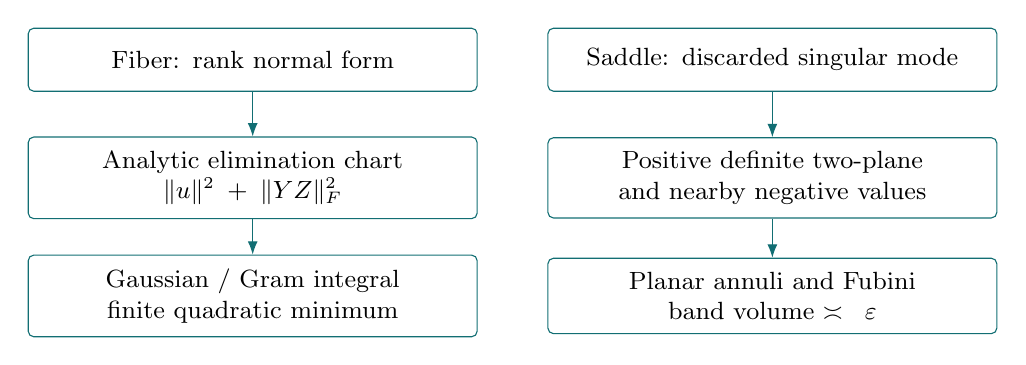
\begin{tikzpicture}[every node/.style={align=center,font=\small},box/.style={draw=accent,rounded corners=2pt,text width=5.35cm,minimum height=0.8cm,inner sep=5pt},>=Latex]
\node[box] (a) at (0,2.2) {Fiber: rank normal form};
\node[box] (b) at (6.6,2.2) {Saddle: discarded singular mode};
\node[box] (c) at (0,.7) {Analytic elimination chart\\$\norm u^2+\Frob{YZ}^2$};
\node[box] (d) at (6.6,.7) {Positive definite two-plane\\and nearby negative values};
\node[box] (e) at (0,-.8) {Gaussian / Gram integral\\finite quadratic minimum};
\node[box] (f) at (6.6,-.8) {Planar annuli and Fubini\\band volume $\asymp\eps$};
\draw[->,accent] (a)--(c);\draw[->,accent] (c)--(e);
\draw[->,accent] (b)--(d);\draw[->,accent] (d)--(f);
\end{tikzpicture}
\end{center}
The local volume calculus transports these estimates back to actual matrix entries.
\src{[B], §§3--10. This is a proof-dependency diagram, not the statement-dependency audit.}
\end{frame}

\begin{frame}[fragile,t,label=slide110]{The local volume calculus}
For nonnegative germs, the pair is unchanged by a local analytic coordinate change with nonsingular derivative, or by comparison $c f\le g\le C f$ with positive constants.

Extra free coordinates do not change the pair. Adding $s$ independent positive quadratic coordinates changes it by
\[
(\lambda,m)\longmapsto(\lambda+s/2,m).
\]
Bounded Jacobian factors affect only the constants in $\asymp$.

\key{The proof must sandwich balls by suitable coordinate boxes.} An informal normal form without control of neighborhoods and Jacobians is not yet a band-volume proof.
\src{[B], §3, local volume calculus. The comparison assertion here is for nonnegative germs, as used on the fiber.}
\end{frame}

\begin{frame}[fragile,t,label=slide111]{The simultaneous rank normal form}
Write $\alpha=a-r$ and $\beta=b-r$. There are decompositions with dimensions
\[
\begin{aligned}
\R^I &: r\;|\;\alpha\;|\;q,\\
\R^H &: r\;|\;\alpha\;|\;\beta\;|\;h,\\
\R^O &: r\;|\;\beta\;|\;p.
\end{aligned}
\]
In suitable bases, $A$ transmits the $r$ and $\alpha$ blocks; $B$ transmits the $r$ and $\beta$ blocks. Only the $r$ block passes through both maps.

Changing bases gives an invertible linear coordinate change on parameter space. Frobenius norms need not be preserved, but remain uniformly comparable.
\src{[B], §4, simultaneous rank normal form.}
\end{frame}

\begin{frame}[fragile,t,label=slide112]{Where the regular dimension comes from}
The derivative of multiplication is
\[
D(BA)_{(A,B)}(\dot A,\dot B)=B\dot A+\dot B A.
\]
Matrices $B\dot A$ form a space of dimension $Ib$; matrices $\dot B A$ form one of dimension $Oa$. Their intersection has dimension $ab$.
Thus
\[
\rk D(BA)=Ib+Oa-ab=s.
\]
The missing output block has dimensions $p\times q$ and size $pq=OI-s$.

The first-order calculation locates the residual obstruction. It does not by itself identify the full higher-order germ.
\src{[B], §§4--5; linearized multiplication and elimination chart.}
\end{frame}

\begin{frame}[fragile,t,label=slide113]{What the elimination chart adds}
The blueprint uses invertible pivot blocks to solve for regular output coordinates and writes an explicit inverse coordinate map.

After those eliminations, the remaining nonlinear block is a smaller matrix product $YZ$. On a sufficiently small neighborhood,
\[
L_\Phi\asymp\norm u^2+\Frob{YZ}^2.
\]
Both chart Jacobians are bounded, and the unused coordinates are free.

\key{This is a statement about the full germ, not only its Hessian or tangent cone.} It reduces the fiber theorem to one residual-origin estimate.
\src{[B], §5, explicit analytic chart, inverse, and loss comparison.}
\end{frame}

\begin{frame}[fragile,t,label=slide114]{Replace the residual volume by a Gaussian Laplace integral}
For $K(Y,Z)=\Frob{YZ}^2$, introduce the finite integral
\[
J_G(T)=\int_{\R^{p\times h}\times\R^{h\times q}}
 e^{-T\Frob{YZ}^2-\Frob Y^2-\Frob Z^2}\,dY\,dZ,
\qquad T\to\infty.
\]
For fixed $Z$, the exponent is quadratic in each row $y_i$ of $Y$:
\[
T\Frob{YZ}^2+\Frob Y^2
=\sum_{i=1}^p y_i(I_h+TZZ^{\mathsf T})y_i^{\mathsf T}.
\]
The matrix $I_h+TZZ^{\mathsf T}$ is positive definite.
\src{[B], §7, steps R1--R2. The Gaussian is an auxiliary analytic device, not a new prior hypothesis in the theorem.}
\end{frame}

\begin{frame}[fragile,t,label=slide115]{Integrate out one matrix exactly}
The scalar Gaussian integral and the real spectral theorem give
\[
\int_{\R^h}e^{-x^{\mathsf T}Mx}\,dx=\pi^{h/2}(\det M)^{-1/2}
\quad(M>0).
\]
Tonelli's theorem then yields
\[
J_G(T)=\pi^{ph/2}\int_{\R^{h\times q}}
 e^{-\Frob Z^2}\det(I_h+TZZ^{\mathsf T})^{-p/2}\,dZ.
\]
All integrations are in the explicitly specified entry measures. This equality is proved, not used as a black-box probabilistic premise.
\src{[B], §7, R1; §6 for the exact measure identities.}
\end{frame}

\begin{frame}[fragile,t,label=slide116]{Eigenvalues expose the singular powers}
Assume $p,q,h>0$. Set $k=\min(h,q)$, $d=\max(h,q)$,
$\eta=(d-k-1)/2>-1$, and $\rho=p/2$.

The eigenvalues $0<s_1<\cdots<s_k$ of the smaller Gram matrix give
\[
J_G(T)=C_{p,q,h}\!\int_{0<s_1<\cdots<s_k}
 e^{-\sum_i s_i}
 \prod_i s_i^\eta
 \prod_{i<j}(s_j-s_i)
 \prod_i(1+Ts_i)^{-\rho}\,ds,
\]
where $0<C_{p,q,h}<\infty$ is independent of $T$.

The Vandermonde factor is the geometric Jacobian. The square case has $\eta=-1/2$, so it must not be discarded as a boundary exception.
\src{[B], §6, exact Wishart/eigenvalue formula; §7, R2--R4.}
\end{frame}

\begin{frame}[fragile,t,label=slide117]{Why the Wishart identity is not a hidden axiom}
The proof develops the real Gram-matrix pushforward and the spectral integration formula with explicit measures and normalizing constants.

Sorting eigenvalues replaces the positive orthant by one ordered chamber. Collision and zero-coordinate walls are null sets; permutation symmetry supplies the factor $k!$.

The final named identity is a theorem used in the proof of \node{answersO77}. Its status must be checked through the complete dependency closure, not inferred from its name.
\src{[B], §6 and §7, R3--R4; Part II certification information.}
\end{frame}

\begin{frame}[fragile,t,label=slide118]{The one-dimensional calculation behind every logarithm}
For $A,\rho>0$, split the integral at $T^{-1}$ and $1$:
\[
\int_0^\infty e^{-x}x^{A-1}(1+Tx)^{-\rho}\,dx
\asymp
\begin{cases}
T^{-A},&A<\rho,\\
T^{-\rho}\log T,&A=\rho,\\
T^{-\rho},&A>\rho.
\end{cases}
\]
On the middle interval, the relevant factor is
\[
T^{-\rho}\int_{1/T}^1x^{A-\rho-1}\,dx.
\]
A logarithm appears exactly at the resonance $A=\rho$.
\src{[B], §7, R5, elementary scalar-integral estimate.}
\end{frame}

\begin{frame}[fragile,t,label=slide119]{From the ordered chamber to a finite minimum}
On the ordered chamber, the Vandermonde is at most $\prod_i s_i^{i-1}$.
A separated subchamber gives a matching lower estimate.

Put $A_i=\eta+i$ for $i=1,\ldots,k$. The result is
\[
J_G(T)\asymp T^{-\nu}(\log T)^\ell,\qquad
\nu=\sum_{i=1}^k\min(A_i,\rho),\quad
\ell=\#\{i:A_i=\rho\}\le1.
\]
The lower bound must retain the logarithmic interval at a resonance; a fixed compact subbox alone would lose that logarithm.
\src{[B], §7, R5, ordered estimate and separated lower regions.}
\end{frame}

\begin{frame}[fragile,t,label=slide120]{The same quadratic reappears}
For $0\le j\le k$, define
\[
B_j=\sum_{i=1}^j A_i+(k-j)\rho
=\frac{j(d-k+j)+p(k-j)}{2}.
\]
Then $\nu=\min_jB_j$. With $t=k-j$ and $\{k,d\}=\{h,q\}$,
\[
2B_j=(h-t)(q-t)+pt=c_{p,q,h}(t).
\]
Thus $\nu=d_0/2$. A resonance gives two adjacent minimizing indices, so $\ell=\mu_0-1$.

\key{The logarithmic multiplicity comes from a tie in a discrete quadratic minimum.}
\src{[B], §7, arithmetic identification after R5.}
\end{frame}

\begin{frame}[fragile,t,label=slide121]{A global Gaussian estimate is not yet a local theorem}
Two further steps are necessary.

First, quartic homogeneity $K(tY,tZ)=t^4K(Y,Z)$ controls Gaussian tails and transfers the order to a Laplace integral on a fixed ball.

Second, the distribution function of $K$ transfers the two-sided Laplace bounds to sublevel-volume bounds:
\[
\int_{B_\delta}e^{-TK}\asymp T^{-\lambda}(\log T)^{m-1}
\quad\Longleftrightarrow\quad
\vol\{K<\eps\}\asymp\eps^\lambda\log(1/\eps)^{m-1}
\]
for the power--log orders established here.

\small The localization and converse estimate are proved in the blueprint; neither is justified merely by writing $T=1/\eps$.
\src{[B], §3, Laplace/sublevel calculus; §7, localization and residual-origin conclusion.}
\end{frame}

\begin{frame}[fragile,t,label=slide122]{Why the minimum-locus formula has a parity correction}
In the balanced global regime, put $\chi=(I+O+H+r)\bmod2$.
The defect identities are
\[
p-q-h=2(a-r)-(I+H-O-r),\qquad
q-p-h=2(b-r)-(O+H-I-r).
\]
If $p>q+h$, the excess above the global minimum is
\[
\Lambda(a,b)-\Lambda_{\min}=\frac{(p-q-h)^2-\chi}{8}.
\]
Hence an odd defect of $1$ still attains the minimum; a larger positive defect does not. The symmetric condition treats $q>p+h$.
The two inequalities become exactly \node{MinimumRankCondition}.
\src{[B], §8, global comparison identities and excess formulas.}
\end{frame}

\begin{frame}[fragile,t,label=slide123]{The saddle proof starts with one discarded mode}
Choose $j>k$, write $(u,v,\sigma)=(u_j,v_j,\sigma_j)$, and perturb
\[
D(x,y)=(xv^{\mathsf T},\ uy^{\mathsf T}),\qquad x,y\in\R^H.
\]
The rung conditions imply the exact identity
\[
L(w+tD)-L(w)=\frac{t^2}{2}Q(x,y)
+\frac{t^4}{2}\langle x,y\rangle^2,
\]
where
\[
Q(x,y)=\norm{Bx}^2+\norm{A^{\mathsf T}y}^2-2\sigma\langle x,y\rangle.
\]
Thus this perturbation sees both a quadratic sign structure and the controlled quartic remainder.
\src{[B], §10, discarded-mode perturbation identity.}
\end{frame}

\begin{frame}[fragile,t,label=slide124]{Why two positive directions are available}
On the $H$-dimensional subspace $(x,y)=(x,-x)$,
\[
Q(x,-x)=\norm{Bx}^2+\norm{A^{\mathsf T}x}^2+2\sigma\norm x^2
\ge2\sigma\norm x^2.
\]
Since $k<r<H$, a nonoptimal rung forces $H\ge2$.
The Hessian therefore has a positive definite two-plane.

Also $\rk(BA)=k<H$, so $B$ has a kernel or $A^{\mathsf T}$ has a kernel. A small cross-perturbation in $Q$ then gives a negative direction, hence lower loss arbitrarily near $w$.
\src{[B], §10, positive two-plane and lower-loss lemmas.}
\end{frame}

\begin{frame}[fragile,t,label=slide125]{The analytic band lemma used at a saddle}
A local analytic estimate proves the following: at a critical point, a positive definite Hessian two-plane together with arbitrarily nearby lower values yields
\[
\vol\{|f-f(w)|<\eps\}\asymp\eps
\]
in every sufficiently small fixed ambient ball.

For the \emph{upper bound}, slice along the two-plane. Uniform strict convexity controls the area of a thin annulus by $C\eps$, uniformly over the transverse parameters.

Integrating those slice estimates gives the full ambient upper bound.
\src{[B], §10, positive-two-plane band estimate. All volumes are locally restricted to fixed balls.}
\end{frame}

\begin{frame}[fragile,t,label=slide126]{Why the lower bound is genuinely ambient}
Nearby lower values produce an open set of transverse slices whose moving convex minimum is below the reference level.

On a smaller fixed region, each such slice contains an annulus of area at least $c\eps$. The transverse set has fixed positive measure.
Fubini then gives the lower bound $c'\eps$ in the ambient ball.

\key{A lower bound on one two-dimensional plane is not enough.} That plane has ambient measure zero; the uniform family of slices is what proves the theorem.
\src{[B], §10, moving center, annulus bounds, and transverse-slice lower estimate.}
\end{frame}

\begin{frame}[fragile,t,label=slide127]{An indefinite Hessian alone would not suffice}
For $f(x,y)=xy$ at the origin,
\[
\vol\{|xy|<\eps\}\asymp\eps\log(1/\eps),
\qquad(\lambda,m)=(1,2).
\]
There is only one positive direction, not a positive two-plane.

At the excluded scalar boundary $I=O=H=r=1$,
\[
L(a,b)-L(0,0)=ab\left(\frac{ab}{2}-\sigma\right),\qquad\sigma>0.
\]
The second factor is a nonvanishing unit near the origin, so this saddle also has pair $(1,2)$.

\small The strict overparameterization assumption is doing real work in the $(1,1)$ conclusion.
\src{[B], §10 and boundary discussion; elementary product-band calculation.}
\end{frame}

\begin{frame}[fragile,t,label=slide128]{Three different things one might verify}
\textbf{Mathematical specification.} Do the definitions and quantifiers express the claim we intend? This was the purpose of Lectures II--IV.

\textbf{Formal derivation.} Is there a kernel-accepted proof term of precisely that type, with only the declared foundational axioms?

\textbf{Artifact and execution.} Did the actual source, dependencies, and checker used correspond to the inspected statement and the claimed run?

Success at one level does not automatically settle the other two.
\src{[B], human-review and certification statements; [Lean-Check], Validating Proofs.}
\end{frame}

\begin{frame}[fragile,t,label=slide129]{What tactics do -- and what the kernel does}
Lean's elaborator resolves notation, implicit arguments, and overloaded operations. Tactics help construct a proof term.

The kernel checks whether that term has the declared proposition as its type. A faulty tactic does not by itself justify accepting an ill-typed proof term.

But the kernel does not compare the proposition with the speaker's informal claim, establish the correctness of an empirical model, or remove every implementation and execution risk.

\key{The crucial human question remains: which proposition was checked?}
\src{[Lean-Elab], Elaboration and Compilation; [Lean-Check], Validating Proofs.}
\end{frame}

\begin{frame}[fragile,t,label=slide130]{The recorded axiom audit}
\leancontext{recorded source guard; not output from a new run}
\begin{lstlisting}[style=lean,basicstyle=\ttfamily\fontsize{8.7}{10.7}\selectfont]
/--
info: 'O77.answersO77' depends on axioms:
  [propext, Classical.choice, Quot.sound]
-/
#guard_msgs (whitespace := lax) in
#print axioms O77.answersO77
\end{lstlisting}

\translation{The recorded dependency list contains propositional extensionality, classical choice, and the quotient soundness axiom.
The guard compares the printed message with the expected message.}
\auditnote{This is the source guard, not a new execution transcript. The separate 7 October replay log is identified on slide~132.}
\src{[B], Part II certification block and reported audits; [Lean-Axioms].}
\end{frame}

\begin{frame}[fragile,t,label=slide131]{Read the three axioms mathematically}
\textbf{Propositional extensionality} ($\node{propext}$): logically equivalent propositions are equal as propositions.

\textbf{Classical choice} ($\node{Classical.choice}$): a nonempty type has a chosen element; no executable selection procedure is required.

\textbf{Quotient soundness} ($\node{Quot.sound}$): equivalent representatives have equal images in the quotient type.

\small This is the reported conventional classical foundation, not an axiom-free proof. An occurrence of \node{sorryAx} would instead indicate an admitted proof; additional axioms would need separate examination.
\src{[Lean-Axioms], Axioms and Computation; [Lean-Check].}
\end{frame}

\begin{frame}[fragile,t,label=slide132]{The checked artifact and the statement review}
\small
The public artifact is \node{O77Full_2026_10_06_20_50_UTC.lean}.
Its SHA-256 is
\par{\fontsize{7.8}{10}\selectfont\ttfamily
54dd6627468f7f1ad19784b8085e567806d0a087095a1f56a99bb920436acacc}.

The 7 October log records successful build status and a separate
\node{leanchecker} module replay. The build used cached results; the replay
used the imported environment, without \node{--fresh}.

The pins are Lean 4.34.0-rc2, commit
\par{\fontsize{7.8}{10}\selectfont\ttfamily 6a10ac8c22beadecabdbb0919c2b50214762f91d},
and Mathlib commit
\par{\fontsize{7.8}{10}\selectfont\ttfamily 664cbbe52927ce6acaa39ca35498336116e123b8}.

Feld's statement review is a separate judgment, reported 17 October.
The 55-module terminal development and seven axiom guards are unchanged.
\src{[B], current review and reproducibility record; repository log \node{recheck-20261007T222112Z-GHTD7O.log}.}
\end{frame}

\begin{frame}[fragile,t,label=slide133]{Reproduce the check with the public package}
From the repository root, unpack the checking package and follow its README
for initial build and setup. Then use the published source:
\par\smallskip
\begin{lstlisting}[style=lean,basicstyle=\ttfamily\fontsize{8.5}{10.5}\selectfont]
tar -xzf o77-local_2026_10_06_22_09_UTC.tar.gz
cd o77-local
./o77.sh build
./o77.sh setup
./o77.sh doctor
./o77.sh recheck ../O77Full_2026_10_06_20_50_UTC.lean
\end{lstlisting}

\small Retain the complete log, source hash, resolved versions, exit statuses,
and axiom output. This is an instruction for reproduction, not a new run.
The package uses rootless Podman; the repository README explains the commands.
\src{\url{https://github.com/nfeld/mais-o77-lean}; [B], current checking record.}
\end{frame}

\begin{frame}[fragile,t,label=slide134]{A useful audit session inside Lean}
\leancontext{after importing or loading the exact development}
\begin{lstlisting}[style=lean,basicstyle=\ttfamily\fontsize{9.3}{11.3}\selectfont]
#check @O77.answersO77
#print O77.AnswersO77
#print axioms O77.answersO77
\end{lstlisting}

\translation{Inspect the fully explicit theorem type, unfold the six-clause contract, and list every axiom in the theorem's proof dependencies.}

For higher assurance, compare against an independently authored trusted statement and use an independent checker where compatible. Imported code and metaprograms should be handled in an isolated environment.

\small The intended mathematical specification is itself part of the trusted input.
\src{[Lean-Check], Validating Proofs; [B], statement-audit package. The commands are instructions, not a transcript of a fresh session.}
\end{frame}

\begin{frame}[fragile,t,label=slide135]{The promised trust slide}
\vspace{0.6cm}
{\Large If you trust Lean\footnote{\verysmall which you should not---blindly},
then you can trust that the claimed theorem is true.}
\vspace{0.55cm}

\key{The precise version:}

If the formal statement means the intended theorem, the inspected source really has the reported checked proof, and its foundational and implementation assumptions are accepted, then that theorem follows.

Lean reduces the burden of checking a long derivation. It does not eliminate the burden of checking the statement or the provenance of the proof.
\src{[B], human-review boundary; [Lean-Check].}
\end{frame}

\begin{frame}[fragile,t,label=slide136]{What the lectures establish -- and what they do not}
\textbf{Mathematics presented:} the all-points fiber formula, every minimizing rank stratum, attained extrema, and the constant pair $(1,1)$ on all specified nonoptimal rungs.

\textbf{Feld's statement review (17 October 2026):} the actual loss, entry measure, band sets, order of limits, finite arithmetic, rank conditions, and six-clause contract express O77 in his judgment.

\textbf{Still separate:} independent reproduction and refereeing, complete personal understanding of the proof, any zeta-pole interpretation beyond the band bounds, and any bridge to SGD or AI safety.

\key{The modest contribution is a precise, auditable geometric answer to a precisely chosen question.}
\src{[B], conclusion and review status; [O77]; [A7], limitations of the proposed bridge.}
\end{frame}

\appendix
\section{Appendix and references}
\renewcommand{\lecturetag}{Appendix}

\begin{frame}[fragile,t,label=slide137]{Appendix: the baseline corollary}
The main theorem already gives the complete answer. Three additional declarations explain the useful statement that ranks $(r,r)$ realize both the least exponent and the largest multiplicity at that exponent.

The next two theorem excerpts are headers with proof bodies omitted, exactly as in the blueprint's statement-audit package.

The subsequent index lists all 42 quoted declarations and their slide locations.
\src{[B], §2.3, baseline-rank corollary and boundary of the statement audit.}
\end{frame}

\begin{frame}[fragile,t,label=declbaselineTwiceLambda]{The baseline candidate is just evaluation}
\leancontext{O77}
\begin{lstlisting}[style=lean]
def baselineTwiceLambda (I O H r : Nat) : Nat :=
  candidateTwiceLambda I O H r r r
\end{lstlisting}
\translation{
\[
\mathrm{baselineTwiceLambda}(I,O,H,r)
=\mathrm{candidateTwiceLambda}(I,O,H,r,r,r).
\]
In ordinary mathematics this equals
\[
r(I+O-r)+d_0(O-r,I-r,H-r).
\]
No existence or extremality is asserted by this definition alone.
}
\src{[B], §2.3; declaration start line(s) 1054.}
\end{frame}

\begin{frame}[fragile,t,label=declbaselineattainedofpairs]{A baseline point attaining the minimum}
\leancontext{O77.Native; theorem header, proof body omitted}
\begin{lstlisting}[style=lean,basicstyle=\ttfamily\fontsize{7.8}{9.8}\selectfont]
theorem baseline_attained_of_pairs {I O H : ℕ} (Phi : RM O I)
    (hPairs : ∀ w : Parameters I O H, w.2*w.1 = Phi →
      HasLocalBandPair Phi w
        ((O77.candidateTwiceLambda I O H Phi.rank w.1.rank w.2.rank : ℝ)/2)
        (O77.candidateMultiplicity I O H Phi.rank w.1.rank w.2.rank))
    (hrH : Phi.rank ≤ H) :
    ∃ w : Parameters I O H, w.2*w.1 = Phi ∧
      w.1.rank = Phi.rank ∧ w.2.rank = Phi.rank ∧
      HasLocalBandPair Phi w ((O77.baselineTwiceLambda I O H Phi.rank : ℝ)/2)
        (O77.candidateMultiplicity I O H Phi.rank Phi.rank Phi.rank) ∧
      IsThresholdMinimizer Phi w
\end{lstlisting}
\translation{
Under the displayed hypotheses, there exists an exact fit of ranks $(r,r)$ carrying the baseline pair and minimizing the exponent, where $r=\rk\Phi$.
}
\src{[B], §2.3; declaration start line(s) 1067.}
\end{frame}

\begin{frame}[fragile,t,label=slide140]{Why hPairs adds no assumption to the main result}
The attainment theorem has an explicit hypothesis: every exact fit carries its candidate pair.

Clause 1 of $\mathrm{AnswersO77}$ supplies precisely this hypothesis. For each exact fit, take $\lambda$ and $m$ to be the candidate values in its biconditional.

The other required bound, $\rk\Phi\le H$, follows from the strict hypothesis $\rk\Phi<H$.

Thus the baseline corollary follows from the main theorem, even though the reusable intermediate attainment theorem has a conditional header.
\src{[B], §2.3, explanation following the baseline theorem header.}
\end{frame}

\begin{frame}[fragile,t,label=declbaselineMultiplicityformula]{The baseline multiplicity is the maximal one}
\leancontext{O77}
\begin{lstlisting}[style=lean,basicstyle=\ttfamily\fontsize{8.2}{10.2}\selectfont]
theorem baselineMultiplicity_formula {I O H r : Nat}
    (hrI : r ≤ I) (hrO : r ≤ O) (hrH : r ≤ H) :
    candidateMultiplicity I O H r r r =
      if (I+O+H+r)%2 = 1 ∧ O+r ≤ I+H ∧ I+r ≤ O+H ∧ H+r ≤ I+O
      then 2 else 1
\end{lstlisting}
\translation{
For $r\le I,O,H$, the candidate multiplicity at ranks $(r,r)$ is $2$ in the odd balanced regime and $1$ otherwise.

This is exactly the value in clause 5. Together with the previous attainment theorem, the same point realizes both extrema.
}
\auditnote{This is a theorem header with its proof body omitted, not a new unproved declaration in the original development.}
\src{[B], §2.3; declaration start line(s) 1086.}
\end{frame}

\begin{frame}[fragile,t,label=slide142]{A compact Lean reading dictionary}
\small
\begin{tabular}{@{}p{.39\textwidth}p{.55\textwidth}@{}}
\toprule
Lean & Reading in this lecture\\\midrule
\node{∀ x, P x} & For every $x$, $P(x)$ holds.\\[6pt]
\node{∃ x, P x} & There exists $x$ satisfying $P(x)$.\\[6pt]
\node{P ∧ Q}, \node{P ↔ Q} & Conjunction; logical equivalence.\\[6pt]
\node{P → Q} & Implication when $P,Q$ are propositions.\\[6pt]
\node{X → Y}, \node{fun x => t} & Function type; function sending $x$ to $t$.\\[6pt]
\node{(x : ℝ)}, \node{.toNat} & A cast/type annotation; conversion to $\N$.\\[6pt]
\node{abbrev}, \node{Type*} & Transparent abbreviation; a type in an inferred universe.\\[6pt]
\node{.1}, \node{.2}, named fields & Projections of a pair or record.\\\bottomrule
\end{tabular}
\src{[B], §2.3 notation guide; [Lean-T].}
\end{frame}

\begin{frame}[fragile,t,label=slide143]{The statement audit stops at a declared boundary}
Every project-defined symbol needed to interpret \node{AnswersO77} has been unfolded in the preceding code slides.

Standard Lean and Mathlib notions remain: real numbers, finite matrix multiplication and rank, finite product measures, scalar logarithms and powers, and order predicates.

The chart maps, Gram densities, and intermediate analytic propositions belong to the proof-dependency graph. They are not extra assumptions hidden in the theorem's type.

\key{A minimal statement audit is not an attempt to reread every definition in Mathlib.} Its trusted-library boundary should nevertheless be explicit.
\src{[B], §2.3, boundary of the statement audit.}
\end{frame}

\begin{frame}[fragile,t,label=slide144]{Statement-audit index 1 / 4}
\fontsize{9}{10.5}\selectfont
\begin{tabular}{@{}p{.54\textwidth}p{.25\textwidth}r@{}}
\toprule
Declaration & Slide(s) & TeX line\\\midrule
\node{RM} & \hyperlink{declRM}{37} & 657\\[2pt]
\node{Parameters} & \hyperlink{declRM}{37} & 659\\[2pt]
\node{frobeniusSq} & \hyperlink{declfrobeniusSq}{38} & 672\\[2pt]
\node{coordinateLebesgue} & \hyperlink{declcoordinateLebesgue}{39} & 676\\[2pt]
\node{matrixLebesgue} & \hyperlink{declmatrixLebesgue}{40} & 680\\[2pt]
\node{entryMeasure} & \hyperlink{declentryMeasure}{41} & 695\\[2pt]
\node{ambientSq} & \hyperlink{declambientSq}{42} & 698\\[2pt]
\node{entryNorm} & \hyperlink{declambientSq}{42} & 701\\[2pt]
\node{loss} & \hyperlink{declloss}{43} & 704\\[2pt]
\node{entryBall} & \hyperlink{declentryBall}{44} & 707\\[2pt]
\node{bandSet} & \hyperlink{declbandSet}{45} & 710\\[2pt]
\bottomrule
\end{tabular}
\par\vspace{5pt}
Slide numbers are clickable. Line numbers refer to the accompanying blueprint, not this Beamer source.
\src{[B], §2.3. All declarations in its displayed audit package are indexed; theorem-header excerpts are identified on their slides.}
\end{frame}

\begin{frame}[fragile,t,label=slide145]{Statement-audit index 2 / 4}
\fontsize{9}{10.5}\selectfont
\begin{tabular}{@{}p{.54\textwidth}p{.25\textwidth}r@{}}
\toprule
Declaration & Slide(s) & TeX line\\\midrule
\node{bandVolume} & \hyperlink{declbandVolume}{46} & 714\\[2pt]
\node{powerLogZeroReal} & \hyperlink{declpowerLogZeroReal}{48} & 739\\[2pt]
\node{powerLogZero} & \hyperlink{declpowerLogZeroReal}{48} & 742\\[2pt]
\node{EThetaZeroPowerLog} & \hyperlink{declEThetaZeroPowerLog}{49} & 745\\[2pt]
\node{RadiusOrder} & \hyperlink{declRadiusOrder}{51} & 763\\[2pt]
\node{HasLocalBandPair} & \hyperlink{declHasLocalBandPair}{54} & 780\\[2pt]
\node{RankData} & \hyperlink{declRankData}{60} & 797\\[2pt]
\node{residualHidden} & \hyperlink{declresidualHidden}{62} & 806\\[2pt]
\node{regularDim} & \hyperlink{declresidualHidden}{62} & 807\\[2pt]
\node{quadratic} & \hyperlink{declquadratic}{67} & 826\\[2pt]
\node{minimumUpTo} & \hyperlink{declminimumUpTo}{69} & 829\\[2pt]
\bottomrule
\end{tabular}
\par\vspace{5pt}
Slide numbers are clickable. Line numbers refer to the accompanying blueprint, not this Beamer source.
\src{[B], §2.3. All declarations in its displayed audit package are indexed; theorem-header excerpts are identified on their slides.}
\end{frame}

\begin{frame}[fragile,t,label=slide146]{Statement-audit index 3 / 4}
\fontsize{9}{10.5}\selectfont
\begin{tabular}{@{}p{.54\textwidth}p{.25\textwidth}r@{}}
\toprule
Declaration & Slide(s) & TeX line\\\midrule
\node{minimizerList} & \hyperlink{declminimizerList}{70} & 833\\[2pt]
\node{residualCost} & \hyperlink{declresidualCost}{66} & 844\\[2pt]
\node{residualQuadratic} & \hyperlink{declresidualQuadratic}{68} & 846\\[2pt]
\node{residualMin} & \hyperlink{declresidualMin}{71} & 850\\[2pt]
\node{residualMinimizerList} & \hyperlink{declresidualMinimizerList}{72} & 853\\[2pt]
\node{residualMultiplicity} & \hyperlink{declresidualMinimizerList}{72} & 856\\[2pt]
\node{candidateTwiceLambda} & \hyperlink{declcandidateTwiceLambda}{73} & 859\\[2pt]
\node{candidateMultiplicity} & \hyperlink{declcandidateMultiplicity}{74} & 862\\[2pt]
\node{IsThresholdMinimizer} & \hyperlink{declIsThresholdMinimizer}{80} & 885\\[2pt]
\node{MinimumRankCondition} & \hyperlink{declMinimumRankCondition}{82} & 899\\[2pt]
\node{globalThresholdFormula} & \hyperlink{declglobalThresholdFormula}{84} & 906\\[2pt]
\bottomrule
\end{tabular}
\par\vspace{5pt}
Slide numbers are clickable. Line numbers refer to the accompanying blueprint, not this Beamer source.
\src{[B], §2.3. All declarations in its displayed audit package are indexed; theorem-header excerpts are identified on their slides.}
\end{frame}

\begin{frame}[fragile,t,label=slide147]{Statement-audit index 4 / 4}
\fontsize{9}{10.5}\selectfont
\begin{tabular}{@{}p{.54\textwidth}p{.25\textwidth}r@{}}
\toprule
Declaration & Slide(s) & TeX line\\\midrule
\node{SingularData} & \hyperlink{declSingularData}{89} & 934\\[2pt]
\node{«prefix»} & \hyperlink{declprefix}{91} & 955\\[2pt]
\node{target} & \hyperlink{decltarget}{92} & 958\\[2pt]
\node{OnRung} & \hyperlink{declOnRung}{93} & 960\\[2pt]
\node{AnswersO77} & \hyperlink{contract1}{99}, \hyperlink{contract2}{100}, \hyperlink{contract3}{101}, \hyperlink{contract4}{102}, \hyperlink{contract5}{103}, \hyperlink{contract6}{104} & 983\\[2pt]
\node{answersO77} & \hyperlink{declanswersO77}{105} & 1031\\[2pt]
\node{baselineTwiceLambda} & \hyperlink{declbaselineTwiceLambda}{138} & 1054\\[2pt]
\node{baseline_attained_of_pairs} & \hyperlink{declbaselineattainedofpairs}{139} & 1067\\[2pt]
\node{baselineMultiplicity_formula} & \hyperlink{declbaselineMultiplicityformula}{141} & 1086\\[2pt]
\bottomrule
\end{tabular}
\par\vspace{5pt}
Slide numbers are clickable. Line numbers refer to the accompanying blueprint, not this Beamer source.
\src{[B], §2.3. All declarations in its displayed audit package are indexed; theorem-header excerpts are identified on their slides.}
\end{frame}

\begin{frame}[fragile,t,label=slide148]{References: the blueprint and the MAIS problem}
\small
\textbf{[B]} GPT Sol 5.6 and GPT Astra 6.0, directed by Niels Feld.
\emph{MAIS-O77 blueprint}, statement-review edition 1.60, 17 October 2026, 15:54 UTC. Accompanying source:
\par\node{mais-o77-blueprint_2026_10_17_15_54_UTC.tex}.

\textbf{[MAIS]} \emph{Math for AI Safety}, research-collaboration repository.
\par\url{https://github.com/Math-for-AI-Safety/MAIS}

\textbf{[O77]} \emph{Learning coefficients on the matrix factorization fiber and saddles}, MAIS-O77. Repository text inspected 12 October 2026.
\par\url{https://github.com/Math-for-AI-Safety/MAIS/blob/main/open-problems/MAIS-O77.md}

\textbf{[A7]} \emph{Effective loss and learning dynamics: selection among the strata of a singular optimal set}, MAIS-A7.
\par\url{https://github.com/Math-for-AI-Safety/MAIS/tree/main/agendas/A7}
\src{MAIS source snapshot: commit 1cb9f003d111ca6de056b18ee574204314c00b8e. Public texts remain drafts; the presentation uses [B] as its mathematical source.}
\end{frame}

\begin{frame}[fragile,t,label=slide149]{References: singular learning theory}
\small
\textbf{[W09]} Sumio Watanabe. \emph{Algebraic Geometry and Statistical Learning Theory}. Cambridge University Press, 2009.

\textbf{[W13]} Sumio Watanabe. \emph{A Widely Applicable Bayesian Information Criterion}. Journal of Machine Learning Research \textbf{14} (2013), 867--897.
\par\url{https://arxiv.org/abs/1208.6338}

\textbf{[AW05]} Miki Aoyagi and Sumio Watanabe. \emph{Stochastic complexities of reduced rank regression in Bayesian estimation}. Neural Networks \textbf{18}(7) (2005), 924--933.

\textbf{[LFWMW23]} Edmund Lau, Zach Furman, George Wang, Daniel Murfet, Susan Wei. \emph{The Local Learning Coefficient: A Singularity-Aware Complexity Measure}. 2023; revised 2024.
\par\url{https://arxiv.org/abs/2308.12108}
\src{Primary sources for the background and prior results; their statistical or zeta statements are not silently added to the formal contract.}
\end{frame}

\begin{frame}[fragile,t,label=slide150]{References: multiplication fibers and public context}
\small
\textbf{[LR24]} Simon Pepin Lehalleur and Rich\'ard Rim\'anyi.
\emph{Geometry of fibers of the multiplication map of deep linear neural networks}. 2024.
\par\url{https://arxiv.org/abs/2411.19920}

For public antecedents and review discussions, the blueprint cites MAIS issues \#3, \#5, and \#12. Attribution in these slides follows the blueprint's account, not a fresh priority determination.
\par\url{https://github.com/Math-for-AI-Safety/MAIS/issues/3}
\par\url{https://github.com/Math-for-AI-Safety/MAIS/issues/5}
\par\url{https://github.com/Math-for-AI-Safety/MAIS/issues/12}

The broader agenda links O77 to O76 (singular SGD limits) and O78 (a time--sample dictionary). Those bridges are not proved by the theorem presented here.
\src{[B], introduction, public-posting credits, and conclusion; [O77] and [A7].}
\end{frame}

\begin{frame}[fragile,t,label=slide151]{References: learning to read Lean}
\small
\textbf{[Lean-T]} \emph{Theorem Proving in Lean 4}. In particular, propositions and proofs, quantifiers, tactics, structures, and type classes.
\par\url{https://lean-lang.org/theorem_proving_in_lean4/}

\textbf{[Lean-Axioms]} \emph{Theorem Proving in Lean 4}, Axioms and Computation.
\par\url{https://lean-lang.org/theorem_proving_in_lean4/Axioms-and-Computation/}

\textbf{[Lean-Elab]} \emph{The Lean Language Reference}, Elaboration and Compilation.
\par\url{https://lean-lang.org/doc/reference/latest/Elaboration-and-Compilation/}

These references explain the language. Their current online version is not the pinned toolchain used for the blueprint's reported check.
\src{Official Lean documentation, consulted for this presentation on 12 October 2026.}
\end{frame}

\begin{frame}[fragile,t,label=slide152]{References: proof validity, meaning, and reproducibility}
\small
\textbf{[Lean-Check]} \emph{The Lean Language Reference}, Validating a Lean Proof.
\par\url{https://lean-lang.org/doc/reference/latest/ValidatingProofs/}

The document distinguishes inspecting a theorem's meaning, checking its proof and axiom dependencies, replaying stored proofs, and comparing with a trusted statement using external checking infrastructure.

The blueprint's pinned Mathlib source is
\par\url{https://github.com/leanprover-community/mathlib4/tree/664cbbe52927ce6acaa39ca35498336116e123b8}

The source extracts quote [B]. This edition records Feld's statement review and the existing 7 October checking log. Updating and typesetting the slides does not constitute another Lean run or independent refereeing.
\src{[B], current review and preservation record; official Lean documentation consulted for the original slides on 12 October 2026.}
\end{frame}

\end{document}
